\documentclass[output=paper]{langscibook}
\ChapterDOI{10.5281/zenodo.15006619}
\author{Yvonne Kathrein\orcid{}\affiliation{University of Innsbruck, Department of German Studies, Tyrolean Dialect Archive}}
\title[On the verticality of lay dialect collections and the attempt to measure it]{„Es werden im wesentlichen [sic!] nur Wörter aufgenommen, welche deutlich unterschiedlich zum Hochdeutschen sind.“: On the verticality of lay dialect collections and the attempt to measure it}

\abstract{Dialect collections created by laypersons not only provide information about the different conditions under which they were created and the associated intentions, but also about how laypersons conceptualize their dialect and try to delimit it “upwards”. Using the example of three selected collections from the Austrian province of Tyrol, the present study shows not only which entries are generally present there, but also how dialectal they are~– taking into account the underlying dialect~– in comparison to the standard language. In doing so, the individual linguistic levels serve as a template according to which the deviations are classified.

It turns out that the collections have about the same amount of special dialect lexis (i.e., lexis that occurs only in the dialects) and about the same amount of entries that differ from the standard language only at the phonological and/or morphological level. However, differences appear in the number of stylistically marked elements and in the calculated $d$-values.

Furthermore, the study shows that the evaluations of the collections can not only be refined by perceptual dialectological methods, but also that the collections can be a good complement to existing perceptual dialectological studies.
}
\IfFileExists{../localcommands.tex}{
  \addbibresource{../localbibliography.bib}
  \usepackage{tabularx,multicol}
%\usepackage{multirow}
\usepackage{subcaption}
\usepackage{url}
\urlstyle{same}

\usepackage{datetime}
\usepackage{enumitem}
\usepackage{langsci-optional}
\usepackage{langsci-lgr}
\usepackage{langsci-branding}

\usepackage{longtable}
\usepackage{xltabular}
\usepackage[linguistics, edges]{forest}
\usepackage{pgfplots}
\pgfplotsset{compat=1.18}
\usetikzlibrary{patterns, tikzmark}
\usepackage{pgfplotstable}
\usepgfplotslibrary{colorbrewer}
\usepackage{listings}
\lstset{basicstyle=\ttfamily,keywordstyle=\normalfont,language=,breaklines=true}

\usepackage{siunitx}
\sisetup{group-digits=none, detect-all=true}

\usepackage{langsci-gb4e}

  \makeatletter
\let\thetitle\@title
\let\theauthor\@author
\makeatother

% Use this Chinese font shipped with TeX Live instead of Source Han, because
% it is more portable/leightweight. Install the "fandol" package from CTAN to
% automatically get this font.
\newfontfamily{\ChineseFandolSong}{FandolSong-Regular.otf}

  %% hyphenation points for line breaks
%% Normally, automatic hyphenation in LaTeX is very good
%% If a word is mis-hyphenated, add it to this file
%%
%% add information to TeX file before \begin{document} with:
%% %% hyphenation points for line breaks
%% Normally, automatic hyphenation in LaTeX is very good
%% If a word is mis-hyphenated, add it to this file
%%
%% add information to TeX file before \begin{document} with:
%% %% hyphenation points for line breaks
%% Normally, automatic hyphenation in LaTeX is very good
%% If a word is mis-hyphenated, add it to this file
%%
%% add information to TeX file before \begin{document} with:
%% \include{localhyphenation}
\hyphenation{
    a-na-ly-sis
    ap-proach-es
    ar-che-o-log-i-cal
    Ar-khan-gelsk
    be-schrei-ben
    Buch-holtz
    Che-lya-binsk
    con-so-nant
    dia-lect
    dia-lect-ology
    Di-a-lekt-for-schung
    Dia-lekt-for-schung
    East-pha-lian
    För-der-ung
    Ge-mein-schaft-lich-keits-ent-wür-fe
    his-tor-i-cal
    Hok-kai-do
    ja-pa-nese
    Ja-pa-nese
    Ka-go-shi-ma
    Ka-li-nin-grad
    Knja-zev
    Ma-kro-be-reich
    Ma-lay-sia
    mor-pho-log-i-cal
    Mos-cow
    Nef-te-yu-gansk
    non-mobile
    nu-cle-ar
    ös-ter-rei-chi-sche
    par-a-digm
    per-zep-ti-ons-lin-gu-is-ti-sche
    plu-ri-zen-tri-schen
    quick-ly
    Reich
    Sax-on
    Schrö-der
    sear-ching
    ste-reo-type
    strength-en-ing
    strong-est
    Stutt-gart
    su-pra-seg-men-tal
    teach-er
    to-po-gra-phy
    To-ron-to
    tra-di-tion-al
    ul-ti-mate-ly
    Um-gangs-spra-che
    Volks-kun-de
    vor-zu-stel-len
    wheth-er
    Wie-sing-er
    with-in
    Wort-at-las
}

\hyphenation{
    a-na-ly-sis
    ap-proach-es
    ar-che-o-log-i-cal
    Ar-khan-gelsk
    be-schrei-ben
    Buch-holtz
    Che-lya-binsk
    con-so-nant
    dia-lect
    dia-lect-ology
    Di-a-lekt-for-schung
    Dia-lekt-for-schung
    East-pha-lian
    För-der-ung
    Ge-mein-schaft-lich-keits-ent-wür-fe
    his-tor-i-cal
    Hok-kai-do
    ja-pa-nese
    Ja-pa-nese
    Ka-go-shi-ma
    Ka-li-nin-grad
    Knja-zev
    Ma-kro-be-reich
    Ma-lay-sia
    mor-pho-log-i-cal
    Mos-cow
    Nef-te-yu-gansk
    non-mobile
    nu-cle-ar
    ös-ter-rei-chi-sche
    par-a-digm
    per-zep-ti-ons-lin-gu-is-ti-sche
    plu-ri-zen-tri-schen
    quick-ly
    Reich
    Sax-on
    Schrö-der
    sear-ching
    ste-reo-type
    strength-en-ing
    strong-est
    Stutt-gart
    su-pra-seg-men-tal
    teach-er
    to-po-gra-phy
    To-ron-to
    tra-di-tion-al
    ul-ti-mate-ly
    Um-gangs-spra-che
    Volks-kun-de
    vor-zu-stel-len
    wheth-er
    Wie-sing-er
    with-in
    Wort-at-las
}

\hyphenation{
    a-na-ly-sis
    ap-proach-es
    ar-che-o-log-i-cal
    Ar-khan-gelsk
    be-schrei-ben
    Buch-holtz
    Che-lya-binsk
    con-so-nant
    dia-lect
    dia-lect-ology
    Di-a-lekt-for-schung
    Dia-lekt-for-schung
    East-pha-lian
    För-der-ung
    Ge-mein-schaft-lich-keits-ent-wür-fe
    his-tor-i-cal
    Hok-kai-do
    ja-pa-nese
    Ja-pa-nese
    Ka-go-shi-ma
    Ka-li-nin-grad
    Knja-zev
    Ma-kro-be-reich
    Ma-lay-sia
    mor-pho-log-i-cal
    Mos-cow
    Nef-te-yu-gansk
    non-mobile
    nu-cle-ar
    ös-ter-rei-chi-sche
    par-a-digm
    per-zep-ti-ons-lin-gu-is-ti-sche
    plu-ri-zen-tri-schen
    quick-ly
    Reich
    Sax-on
    Schrö-der
    sear-ching
    ste-reo-type
    strength-en-ing
    strong-est
    Stutt-gart
    su-pra-seg-men-tal
    teach-er
    to-po-gra-phy
    To-ron-to
    tra-di-tion-al
    ul-ti-mate-ly
    Um-gangs-spra-che
    Volks-kun-de
    vor-zu-stel-len
    wheth-er
    Wie-sing-er
    with-in
    Wort-at-las
}

  \togglepaper[1]%%chapternumber
}{}
\keywords{dialect collections, lay dialect concepts, dialectality values, Levenshtein, perceptual dialectology}

\begin{document}
\graphicspath{{figures/kathrein}}
\maketitle
\label{chap:kathrein}
% ATTENTION: Diacritics on the following phonetic characters might have been lost during conversion: {'ɪ', 'ʉ', 'ɔ', 'ə', 'ɛ'}

\section{Introduction}
\label{sec:kathrein:1}
In recent years we have noticed an increasing number of online dialect collections created by laypersons. These word lists with ``translation", often compiled in years of work by several dialect-speaking and -interested persons, mostly have the purpose to save dialectal words and phrases from being forgotten. But also – from the laypeople's point of view – the special characteristics of the respective dialect are documented in this way.

Such collections have received little scholarly attention, not least because their compilation does not stand up to scientific criteria: The expertise of the collectors is based primarily on the fact that they are dialect speakers of the dialect being documented. This also means that the entries in the collections were selected mainly by self-observation rather than by word research based on a fixed questionnaire: The collectors themselves considered which words of a particular dialect might be worth recording. 

I am not talking about dialect dictionaries that were compiled by experts such as the “Wörterbuch der Bairischen Mundarten in Österreich (WBÖ)”, the “Bayerisches Wörterbuch (BWB)” or the “Schweizerisches Idiotikon”; all of them are long-term projects with a duration of more than a hundred years (cf. \citealt{Stöckle2020, SchnabelEtAl2020, LandoltRoth2020}). Of course, laymen were and are significantly involved in their compilation, e.g. by responding to the calls of the respective dictionary commissions and answering the questionnaires sent to them, sometimes even over a period of years. (cf. \cites[vii--viii]{DollmayrKranzmayer1963}[144]{LandoltRoth2020}[v, xi--xiv]{DenzEtAl2002}) A more recent method of involving the public is to respond to online questionnaires. (cf. \citealt{Retti1999, HoferMeier2015}). In any case, however, standardized questionnaires developed by scientists are used, among other instruments, to collect material.

This does not apply to those collections that will be discussed here: I am talking about collections (and not dictionaries) that have been created in bottom-up processes involving (almost) exclusively linguistic laypersons, i.e., people interested in local history or people enthusiastic about their dialect, either as individuals or as a group. And they have collected their material, as I said, not by (standardized) questionnaires, but by self-observation, which has led to more or less mature collections without any claim to completeness (on the qualitative spectrum cf. \sectref{sec:kathrein:2} as well as \cite{Eickmans1980}).

But it is precisely this incompleteness, this non-systematicity, this non-sci\-en\-ti\-fi\-city, this lay idea of one’s own dialect that is of interest. And I see this in the interest of perceptional dialectology. Although the question of how laypeople conceptualize dialect(s) is central to this relatively new field of dialectology, lay dialect collections have not been considered so far. This is surprising because such collections involve issues of salience as well as the spatial extension of dialects. And these, in turn, are central concepts of perceptual dialectology (for the spatial, horizontal dimension cf. e.g. \citealt{Diercks1988, Auer2004, LameliEtAl2008, Anders2008, Preston2010, Hundt2010, Schröder2019}; for salience cf. e.g. \citealt{Lenz2010, Purschke2011, Purschke2014, Auer2014, AndersEtAl2014, ElmentalerEtAl2010, PalliwodaSchröder2016, Hettler2018}).

However, the spatial dimension to which perceptual dialectology has been devoted so far needs to be expanded, in my opinion: It is not only about the spatial, namely the horizontal, extension of dialect(s), but also about how laypeople understand the vertical dimension. And here, layperson’s dialect collections are an almost predestined source: They have to deal with the question whether individual entries are still dialect at all or whether they already belong to a more widely used, supra-regional, colloquial variety – perhaps even a standard variety. And thus, they also touch on a question that has existed since the first lay linguistic studies, namely the question of the interweaving of “subjective” and “objective” material, i.e. the material obtained by laypeople and the material processed by scientists (cf. \citealt{Preston1999}).

The present study is thus a first attempt to approach these lay collections from what I understand, with reference to the above remarks, to be a perceptual dialectological standpoint. It aims at evaluating a sample of three inner-Alpine online lay collections with regard to a) their content and b) their dialectality, or in other words, it addresses the question to what extent the entries differ from the standard language and how one could methodically proceed to measure these deviations.

\section{Dialect collections of laypersons}
\label{sec:kathrein:2}
As outlined above, the dialect collections of laypersons are currently experiencing a renaissance, at least it seems so, as we can observe a large number of them appearing on the Internet (but also in printed form) presenting different types of data, namely: 

\begin{itemize}
\item the local vocabulary of {geographic units} such as 
\begin{itemize}
\item a single {place} (e.g. Außervillgraten\footnote{\url{https://ausservillgraten.tirol.gv.at/kultur/villgraterisch} (Accessed 21 November, 2022)} or Lustenau\footnote{\url{https://www.lustenau.at/media/209/download/mundartdatei.pdf?v=1} (Accessed 21 November, 2022)}), 
\item a {valley} (e.g. Zillertal\footnote{\url{https://www.zillertaler-woerterbuch.com/} (Accessed 21 November, 2022)} or Vinschgau\footnote{\url{http://www.chrizia.com/c_ling_wbvd_abc.htm} (Accessed 21 November, 2022)}) 
\item or a larger historically developed {region} (e.g. Burgenland\footnote{\url{https://mundart-burgenland.at/woerterbuch.php?lang=hianzisch & char=A} (Accessed 21 November, 2022)}, Bavaria\footnote{\url{https://www.bavariastore.de/bayerische-mundart/} (Accessed 21 November, 2022)} or the former region Baden\footnote{\url{https://freiburg-schwarzwald.de/alemannisch/badisch-deutsch.htm\#Badisch\%20-\%20Deutsch\%20-\%20\%C3\%9Cbersetzer} (Accessed 21 November, 2022)}), 
\end{itemize}
\end{itemize}

or they present 
\begin{itemize}
\item the vocabulary of a {linguistic} {unit} (e.g. “Fränkisch”\footnote{\url{https://aus-meinem-kochtopf.de/fraenggisch-werdderbuch-woerterbuch-fraenkisch-deutsch/} (Accessed 21 November, 2022)}, “Bodenseealemannisch”\footnote{\url{https://www.alemannisch.de/eip/pages/seealemannisch.php} (Accessed 21 November, 2022)}) 
\end{itemize}

or
\begin{itemize}
\item a {combination} of both (e.g. “Hegau-Alemannisch”\footnote{\url{https://www.staff.uni-mainz.de/pommeren/Miszellen/Alemannisch.html} (Accessed 21 November, 2022)}) 
\end{itemize}

as well as
\begin{itemize}
\item the vocabulary of (former) groups (e.g. Walser\footnote{\url{http://www.walser-alps.eu/mundart/woerterbuch} (Accessed 05 December, 2022)}).
\end{itemize}

The collections are accessible on the Internet in different ways: They exist either as a stand-alone website or are integrated as a subpage in a parent page. These higher-level pages can in turn be very different. They range from official community websites to sites of clubs and customs groups, tourism associations, music groups, hotels and guesthouses, etc., up to personal sites. They can be found as a separate element in the sitemap or – somewhat hidden – in a blog post or as a pdf. Although search engines react differently to searches for such collections, in most cases the search leads quickly to a result, even if the name of the page reflects the dialectal pronunciation of the respective dialect (e.g. “Sainihånserisch” for the dialect of St. Johann in Tyrol (Austria), “Muntafuner Dialekt” for the dialect of the valley Montafon in Vorarlberg (Austria) or “Soorser Wöörterbüechli” for the dialect of Sursee (Switzerland)).

As can be concluded from the various operators of the websites, the target audience is equally diverse. It can be locals who speak the respective dialect themselves, it can be people who are interested in the respective dialect in general, but it can also be (temporary) immigrants or guests. On the one hand, these collections are intended to inform them about the respective dialect and its peculiarities. This also includes enabling the smoothest possible communication between “ingroup” and “outgroup” (whether it is really possible or not\footnote{For example, there is an extensive collection of words used in (Upper) Austria to facilitate communication between foreign and local students: \url{http://www.fim.uni-linz.ac.at/Woerterbuch_oesterr_deut_englisch.htm} (Accessed 5 December, 2022)}). On the other hand, self-expression, the presentation of the curious, the incomprehensible, the unpronounceable, the comical is also more or less present; this is especially the case with those collections that are specifically aimed at tourists.

As for the history of their creation, the collections are the work of a single person or, more often, the work of several people who compile idioms/dialectalisms over a certain period of time (which can be years). They usually have predecessor collections as a basis on which new words and expressions are added. Publication on the Internet sometimes makes it possible to participate in the collection if one knows the dialect in question. This also means that the authorship is not always traceable.

It goes without saying that due to this heterogeneous process, the collections vary in length, quality, content and presentation. At the macro level, the vocabulary is usually presented in two columns (as in a vocabulary book), with a bar at the top or bottom of the page that allows navigation between letters (see \figref{fig:kathrein:1}). Furthermore, navigation can be enabled by a search function (see \figref{fig:kathrein:2}). However, the content can also be organized into topics, similar to an onomasiological dictionary (see \figref{fig:kathrein:3}).

  
\begin{figure}
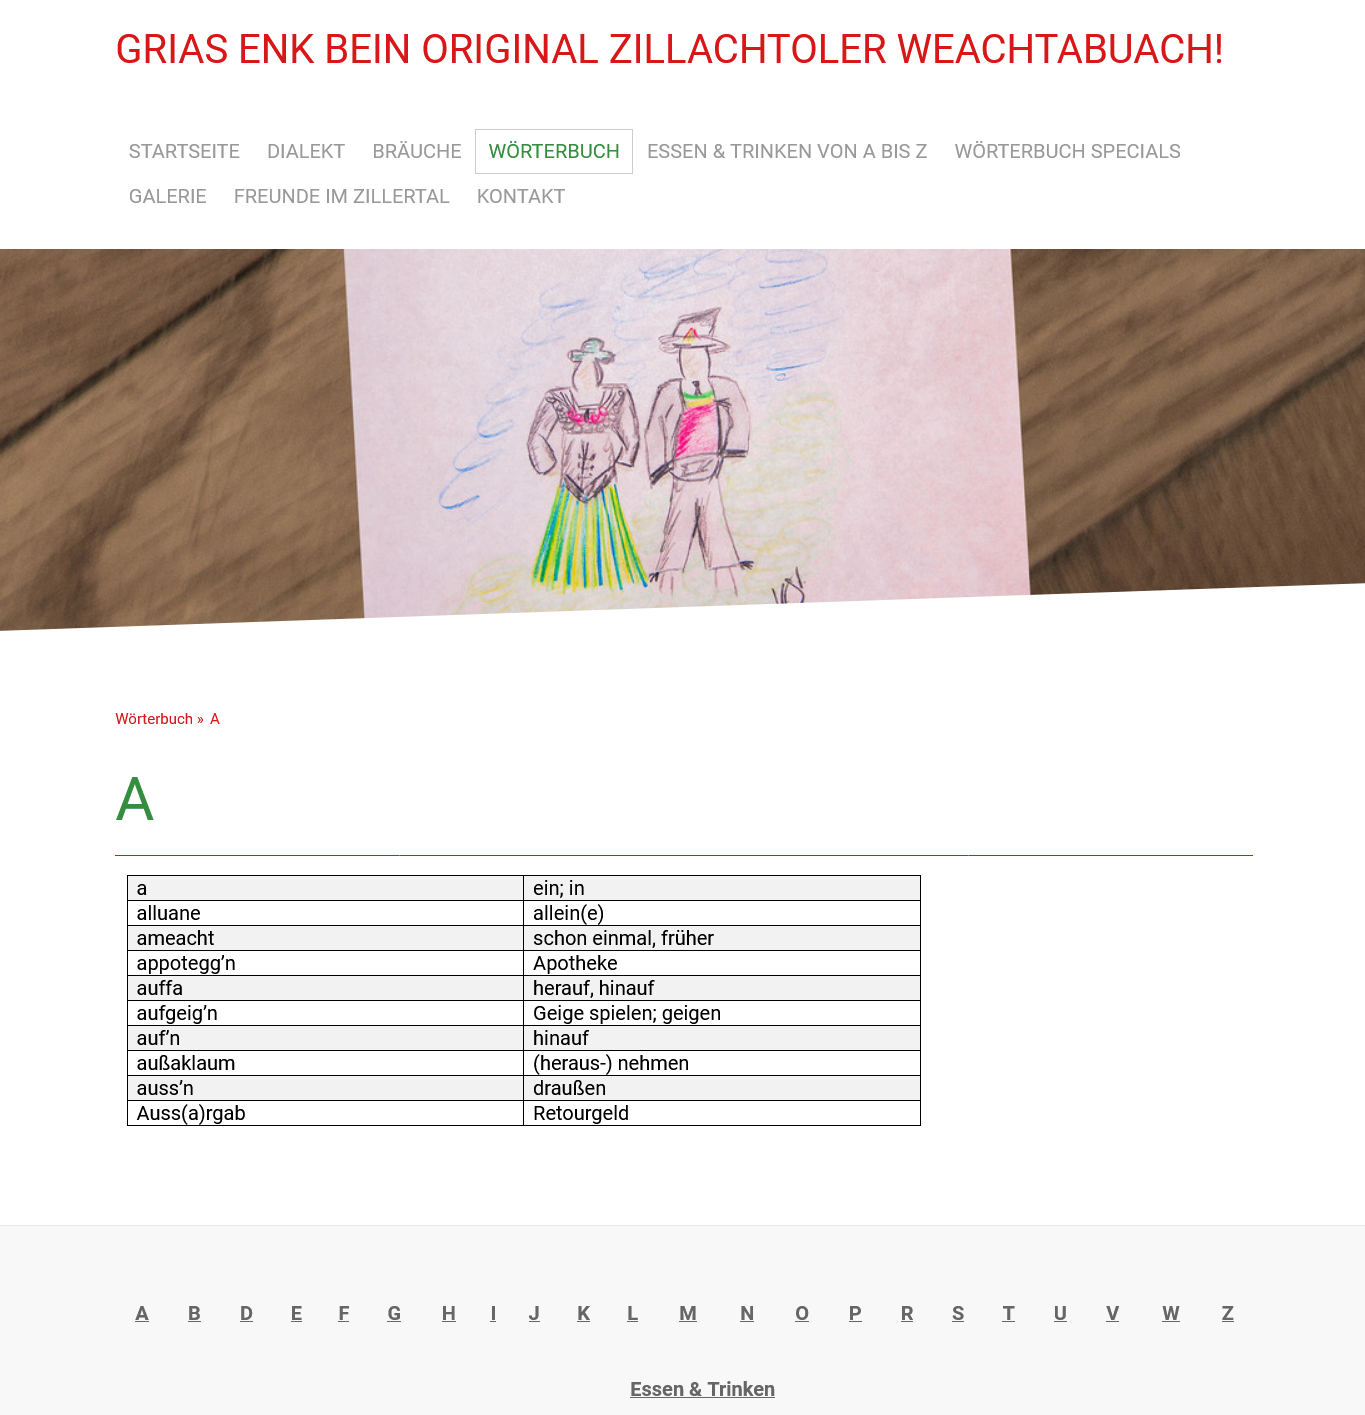
\includegraphics[width=\textwidth]{KathreinLaydialectcollectionsrevised-img001.png}
\caption{\label{fig:kathrein:1}The collections may be quite rudimentary such as the “Original Zillachtoler Weachtabuach” [“Original dictionary of the Ziller valley”, author’s translation] } 
\end{figure}

\begin{figure}
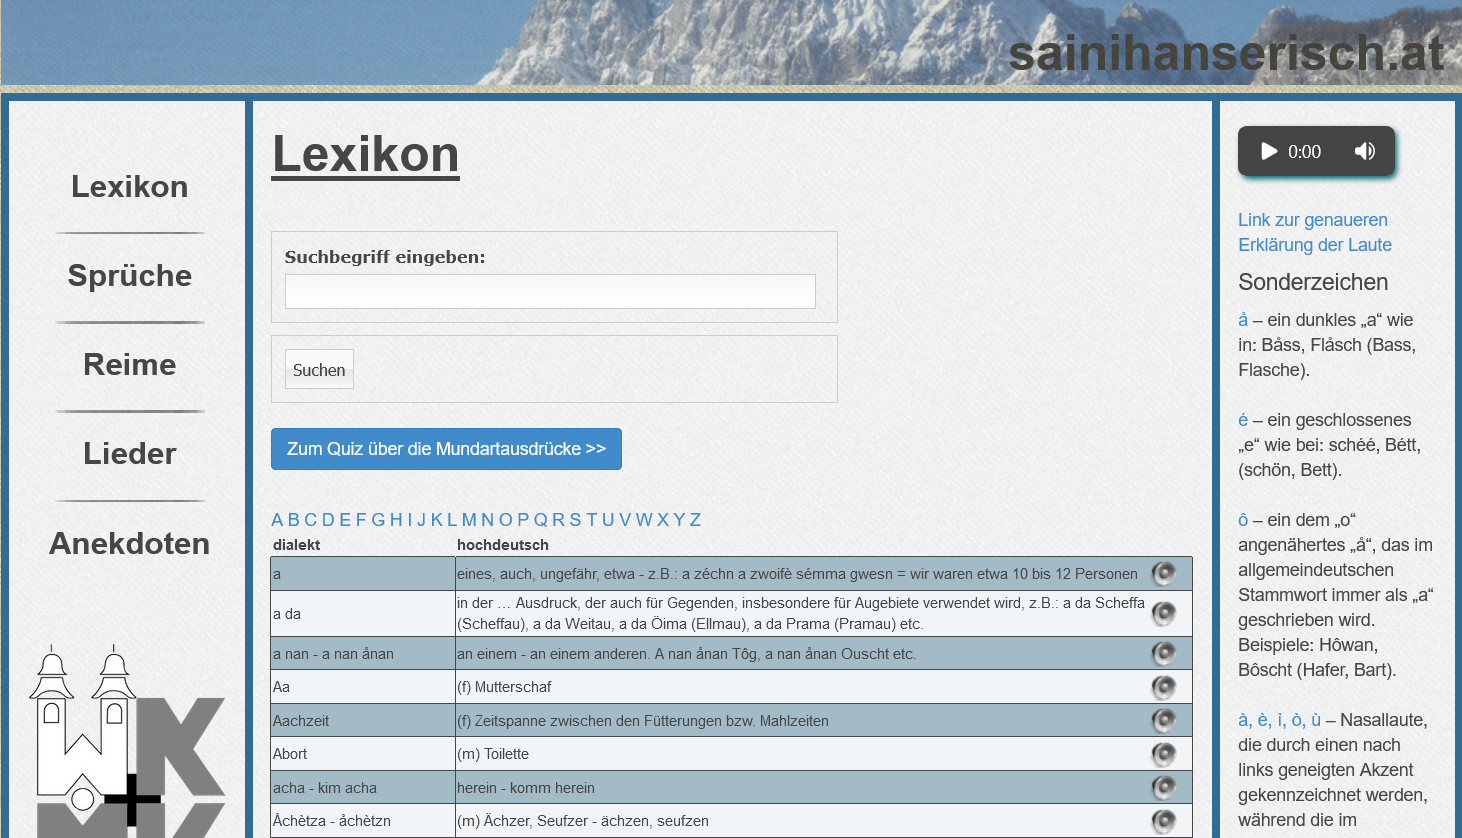
\includegraphics[width=\textwidth]{KathreinLaydialectcollectionsrevised-img002.png}
\caption{\label{fig:kathrein:2} A search function that allows searching for dialect words as well as the Standard German translation, an alphabetical bar, a two-column outline, audio examples and information on transcription: The St. Johann in Tirol collection is in many parts more sophisticated than others (\url{https://www.sainihanserisch.at/lexikon.html})}
\end{figure}

\begin{figure}
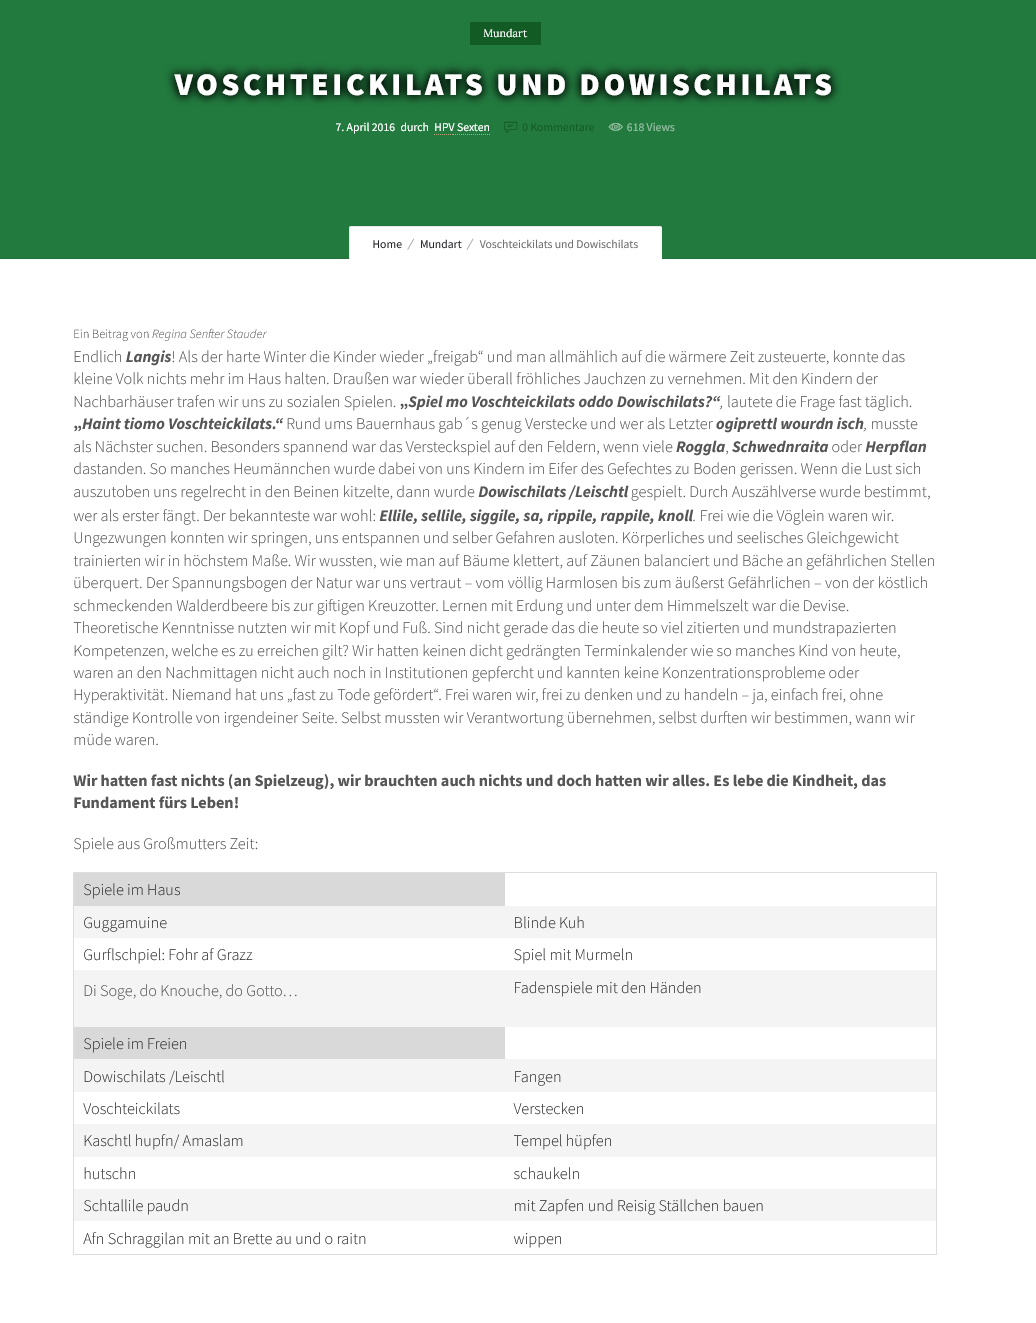
\includegraphics[width=\textwidth]{KathreinLaydialectcollectionsrevised-img003.png}
\caption{\label{fig:kathrein:3} The local vocabulary presented in subject areas, here “Voschteickilats und Dowischilats” [“hide and catch”, author’s translation], introduced by a text about children’s games on the website of the monument protection association of Sexten (South Tyrol/Italy) (\url{http://heimatpflege-sexten.eu/voschteickilats-und-dowischilats/})}
\end{figure}

At the micro level, entries may simply consist of the dialect word or phrase with a more or less strict transcription – usually using at least some diacritics – and the translation without any other additional information (see \figref{fig:kathrein:1}). They may contain grammatical information and/or syntactic context if this seems necessary, as well as audio and/or visual material (see \figref{fig:kathrein:2}), sometimes even information on (presumed) etymology.\footnote{For example in a collection called “Allgäuer Wörterbuch” (\url{https://www.dein-allgaeu.de/regionen/regionen_woerterbuch_a.html}) or the “Wörterbuch ‘Schriftdeutsch – Alemannisch’” (\url{http://hausen.pcom.de/kultur_bildung/olschowka/w\%C3\%B6bu_schrd_alem_start.htm}) (both accessed 5 December, 2022)} In addition, the collections are often supplemented by dialectal idioms, rhymes and phrases, and sometimes by local names.

This is not an exhaustive description of the different forms of presentation and contents of the individual collections. The description merely gives a small insight into the variety and diversity of amateur dialect collections.

\section{Methods: Preparation of a corpus and evaluation procedure}
\label{sec:kathrein:3}
\subsection{Choosing the collections}
\label{sec:kathrein:3.1}
For this paper, three lay collections from the Austrian province of Tyrol were selected (see \figref{fig:kathrein:4}). All of them are accessible via the Internet.

They were selected according to their geographical distribution and their information content: The dialects should be clearly distinguishable from each other (see \figref{fig:kathrein:5} for the dialect regions) and the collections should allow at least a broad phonetic transcription of the individual entries by providing audio material. 


\begin{figure}
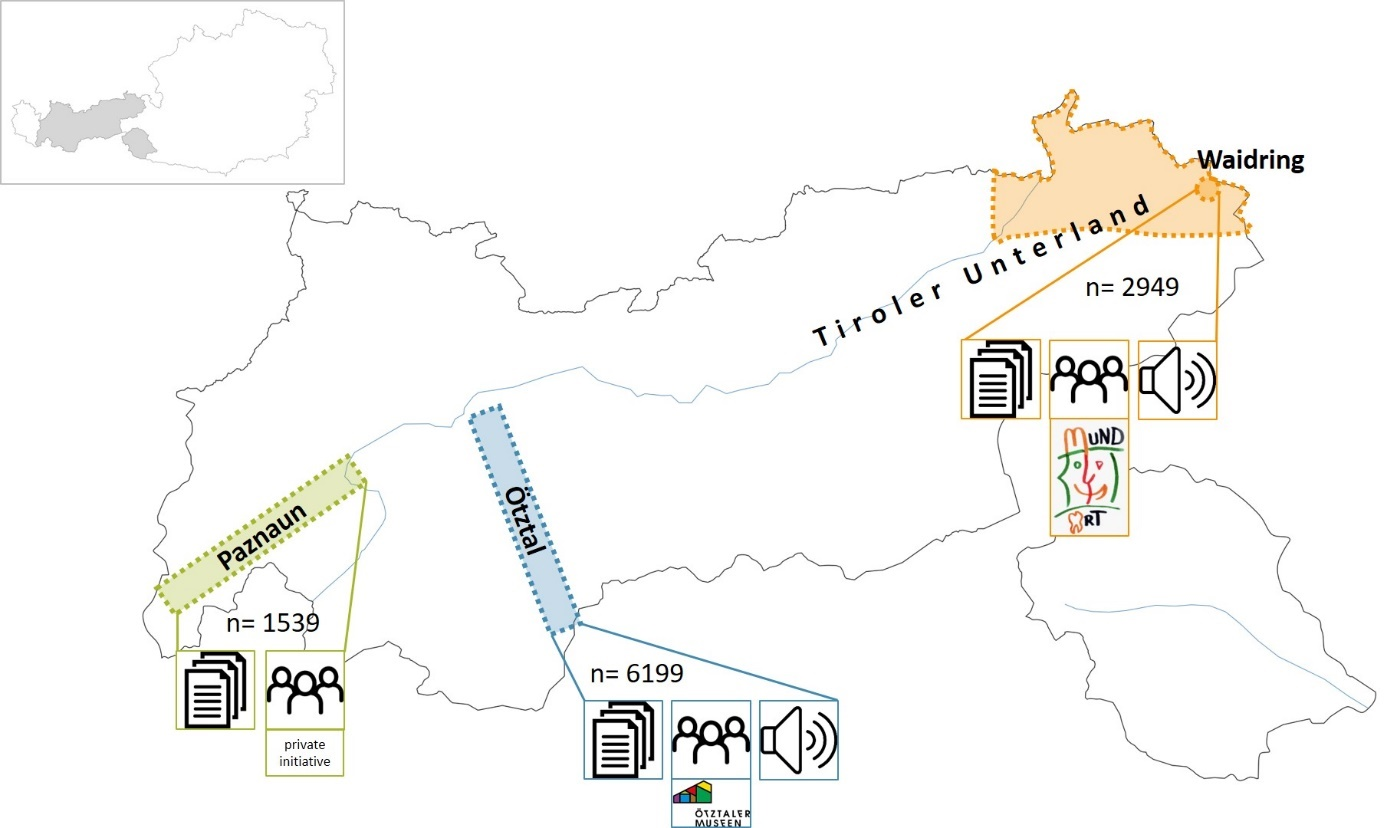
\includegraphics[width=\textwidth]{KathreinLaydialectcollectionsrevised-img004.jpg}
\caption{\label{fig:kathrein:4} Three collections from three different regions in Tyrol were chosen.
(Underlying map created by Y. Kathrein with SprachGIS – \url{regionalsprache.de})}
\end{figure}

\begin{figure}
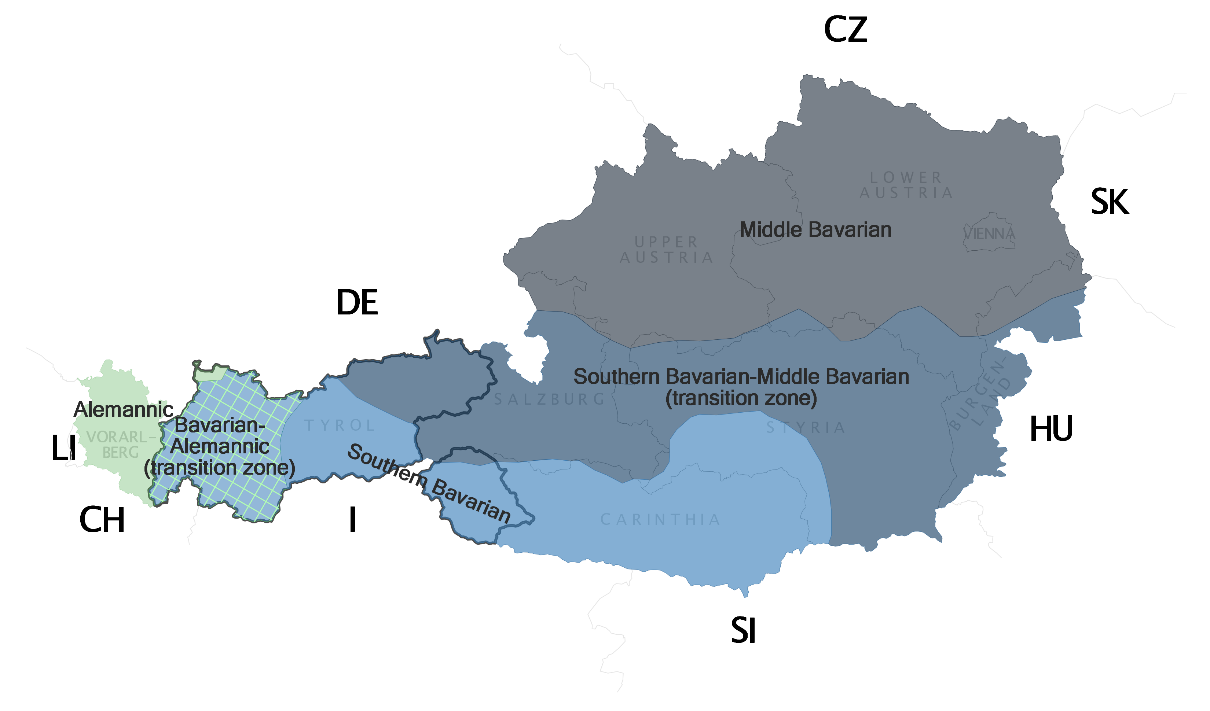
\includegraphics[width=\textwidth]{KathreinLaydialectcollectionsrevised-img005.png}
\caption{\label{fig:kathrein:5} Dialect regions in Austria according to \cite{Wiesinger1983}. The borders of Tyrol are highlighted. (Map created by Y. Kathrein with SprachGIS – \url{regionalsprache.de})}
\end{figure}

\subsubsection{The Paznaun collection}
\label{sec:kathrein:3.1.1}
On the western border of the province of Tyrol lies the Paznaun valley. The variety spoken there is assigned to Southern Bavarian, but is also quite strongly interspersed with Alemannic, since the Paznaun valley borders on the western province of Vorarlberg, whose dialects are Alemannic (see \figref{fig:kathrein:5}) (cf. \citealt[836--842]{Wiesinger1983}).


As shown in \tabref{tab:kathrein:1}, the dialect differs from Alemannic mainly in that mhg. \textit{a} is raised to /ɔ/ (mhg. \textit{g}\textbf{\textit{a}}\textit{bele} > dial. /g\textbf{ɔ}blɐ/ ‘fork’) in all positions, the umlauts are delabialized (mhg. \textit{h}\textbf{\textit{ä}}\textit{chel} > dial. /h\textbf{a}xlɐ/ ‘picking tool for blueberries’) and the mhg. diphthongs \textit{î}, \textit{û} and \textit{iu} are diphthongized (New High German diphthongization) (cf. \citealt[830--831]{Wiesinger1983}). Alemannic features are nevertheless present; for the phonetic domain, this applies, for example, to mhg. \textit{ou}, which is preserved as /oː/ or /ou/ (cf. \citealt[831, 837]{Wiesinger1983}). Thus, mhg. \textit{b}\textbf{\textit{ou}}\textit{m} is realized as /p\textbf{oː}m/. A peculiarity of the dialect in Paznaun (and in the neighboring Stanzertal to the north) is the treatment of mhg. \textit{ei} as /aː/ (cf. \citealt[837]{Wiesinger1983}) as in dial. /p\textbf{aː}/ for mhg. \textit{b}\textbf{\textit{ei}}\textit{n} ‘bone’, which Kranzmayer regards as a “bavarianization of that older \textit{ǟ}, as spoken for mhg. \textit{ei} beyond the Arlberg pass in Montafon and in the Klostertal [...].” (\cite[60]{Kranzmayer1956}, §20g4) [author’s translation]. A common feature with Alemannic is also found in the treatment of the final -\textit{en} in words like \textit{gelog}\textbf{\textit{en}} (‘lied’ (past participle of \textit{lie})). It appears as /ɐ/ (/glo\textbf{ː}g\textbf{ɐ}/). (cf. \cites[22, 92]{Schatz1903}[115(§46h1)]{Kranzmayer1956}) 

\begin{table}
\fittable{\begin{tabular}{lllll}
\lsptoprule
{mhg.} & {mhg. example} & {Paznaun} & {example from collection} & {Alemannic}\\
& & & & (Montafon) \\
\midrule
{\textit{a}} & \textit{g}\textbf{\textit{a}}\textit{bele} & {/ɔ/} & /g\textbf{ɔ}blɐ/ ‘fork’ & {/a/}\\
\midrule
{\textit{ä}} & \textit{h}\textbf{\textit{ä}}\textit{chel} & {/a/} & /h\textbf{a}xlɐ/ ‘picking tool for blueberries’ & {/ɛ/}\\
\midrule
\textit{î} & \textit{k}\textbf{\textit{î}}\textit{f} & {/ai/} & /kx\textbf{ai}f/ ‘tight’ & {/iː/}\\
\textit{iu} & \textit{sch}\textbf{\textit{iu}}\textit{ch}  & {/ui/} & /ʃ\textbf{ui}x/ ‘shy’ & \textbf{/yː/} \\
\textit{û} & \textit{str}\textbf{\textit{û}}\textit{che} & \textbf{/au/} & /ʃtr\textbf{au}xɐ/ ‘chill’ & \textbf{/uː/}\\
\midrule
{\textit{ou}} & \textit{b}\textbf{\textit{ou}}\textit{m} & {/oː/,} {/ou/} & /p\textbf{o}ːm/ ‘tree’ & {/o/}\\
\midrule
{\textit{ei}} & \textit{b}\textbf{\textit{ei}}\textit{n} & {/aː/} & /p\textbf{aː}/ ‘leg, bone’ & {/eː/}\\
\midrule
{\textit{-en}} & \textit{gelog}\textbf{\textit{en}} & {/ɐ/}  & /gloːg\textbf{ɐ}/ ‘lied’ & {/ɐ/}\\
\lspbottomrule
\end{tabular}}
\caption{\label{tab:kathrein:1}Dialect features of the Paznaun valley in contrast to the Alemannic dialect in the adjacent Montafon region}
\end{table}
\clearpage

Since 2011 there is an online collection for the Paznaun valley\break(\url{http://paznaunerisch.at}). With 1539 entries (as of August 2, 2021) it is the smallest collection to be analyzed here. It is based on several preliminary analogue works, mainly carried out by three persons: a retired elementary school principal, a retired elementary school teacher and the former valley doctor. This analog material was made available online to the general public and expanded by three private persons from this valley. People who speak the Paznaun dialect can contribute to the collection themselves by sending their words to those responsible. The contributions will then be checked and integrated into the collection. 

The entries are presented on a single Wiki page (see \figref{fig:kathrein:6}). Links for alphabetical search and two columns with the dialect word on the left and the translation on the right side make it quite a simple collection. In some cases, it is indicated in which part of the valley the word is used. In addition, there is sometimes information on whether the word is already disappearing (e.g. \textit{āperlig}, \textit{āperli} ‘poor (rather forgotten in the upper valley, still used in the lower valley)’ [author’s translation]), in which contexts it is used (e.g. \textit{ausrucka} ‘to move out (concerning the music band, the rifle company)’ [author’s translation], or how it is used stylistically (e.g. \textit{an Schråga} `a wooden frame; derogatory for an ugly person') [author’s translation]. As I myself am a native speaker of the dialect spoken in the Paznaun valley, I was able to transcribe the items phonetically although the site does not provide audio material.

 

\begin{figure}
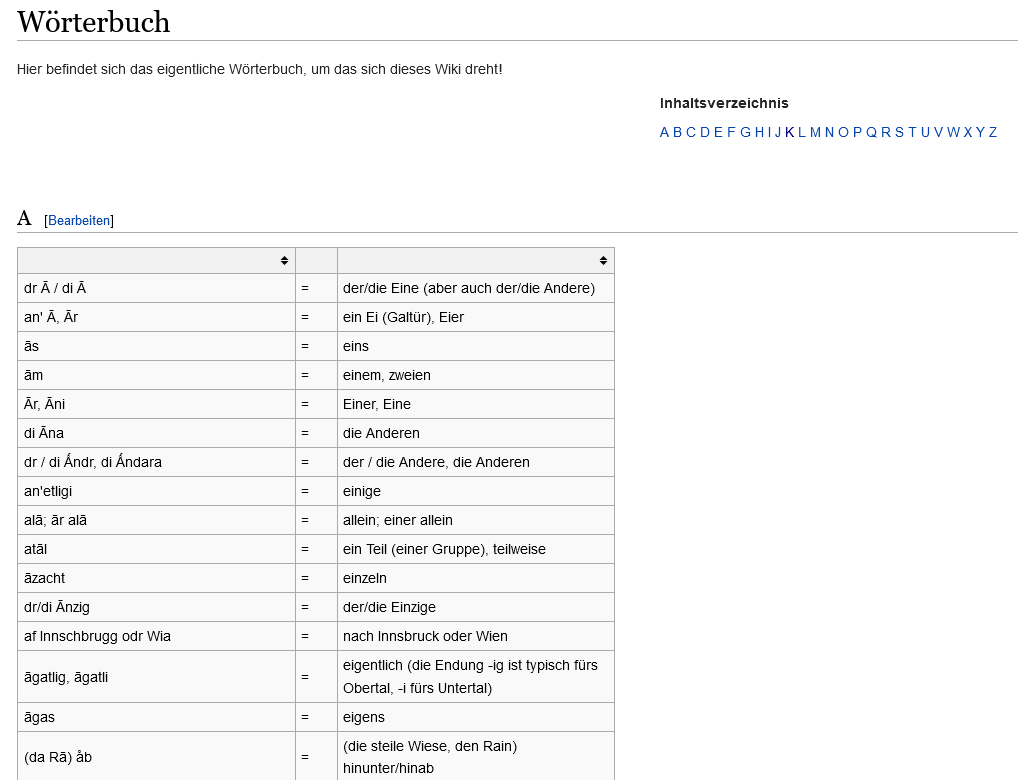
\includegraphics[width=\textwidth]{KathreinLaydialectcollectionsrevised-img006.png}
\caption{\label{fig:kathrein:6} The collection from the Paznaun valley is kept very simple: It only consists of links for alphabetical search and two columns.}
\end{figure}

The Wiki is intended to a) serve as a reference work for the Paznaun dialect and its peculiarities\footnote{“Diese Wiki soll als kleines Nachschlagswerk für diesen Dialekt und seine Eigenheiten dienen.” [‘This wiki should serve as a small reference work for this dialect and its peculiarities.’; author’s translation]} and b) document words that are about to disappear.\footnote{“Viele Wörter [sic!] die mit der Zeit verloren/vergessen wurden, können so einfach nachgeschlagen werden.“ [‘Many words that have been lost/forgotten over time can be easily looked up this way.’; author’s translation]} Whether this also means that the collectors want to preserve the dialect and thus carry it into the future, so that it strengthens again, is not entirely clear. In any case, however, this circumstance resonates when the three editors explain that the preservation of the dialect is close to their hearts.\footnote{“Uns allen lag und liegt die Erhaltung des Dialekts am Herzen. Da sich die Welt im Tal aber gründlich geändert hat, ist heute schon vieles nicht mehr im Gebrauch. Somit ist einiges aus der alten Zeit hier zumindest konserviert.“ [‘The preservation of the dialect was and is close to all our hearts. However, since the world in the valley has changed thoroughly, many things are no longer in use today. Thus, some of the old time is at least preserved here.’; author’s translation]}

\subsubsection{The Ötztal collection}
\label{sec:kathrein:3.1.2}
The second collection concerns the Ötztal that lies further east (see \figref{fig:kathrein:4}). It is also located in the Southern Bavarian-Alemannic transition area (see \figref{fig:kathrein:5}). Unlike in Paznaun, however, the final -\textit{en} is realized as /n/ or /ŋ/ rather than as a vowel, so that it becomes /moxn̩/ (‘to make’) and /ge̞ˈlɵːgŋ/ (‘lied’) (cf. \citealt[22, 92]{Schatz1903}). Another phonetic characteristic concerns the palatal pronunciation of mhg. \textit{o} and \textit{uo}, for instance in \textit{Loch} (dial. /lɵç/) (‘hole’) or \textit{gut} (dial. /gʉət/) (‘good’), especially in the middle communities of the valley (cf. \citealt{KleinEtAl1965}: K. 30, 51).

At the morphological level, the following characteristics should be mentioned: the preservation of final short vowels, such as dial. /bete̞/ vs. std. /be̞t/ (‘bed’), /siɐse̞/ vs. std. /syːs/ (‘sweet’) or /fiɐse̞/ (‘feet’), whose \textit{e} has been apocopied in other dialects (cf. \citealt[49, 93]{Schatz1903}), and the preservation of the schwa sound in the prefix \textit{ge}{}- before \textit{h}, \textit{w}, liquids, nasals, and plosives (/ge̞hɛɐʀn/ ‘to belong’, /ge̞veːsn̩/ ‘have been’, /ge̞ˈlɵːgŋ/ ‘lied‘, /ge̞moxe̞t/ ‘have made’, /\textbf{ge̞}plɛɐxt/ ‘cried’) (cf. \citealt[85]{Kranzmayer1956}, §29e).

\begin{table}
\begin{tabular}{llll}
\lsptoprule
{ mhg.} & {mhg. example} & { Ötztal} & { example from collection}\\
\midrule
{ \textit{-en}} & \textit{mach}\textbf{\textit{en}} & /n/ & /mox\textbf{n̩}/ ‘to make’\\
& \textit{gelog}\textbf{\textit{en}} & /ŋ/ & /ge̞ˈlɵːg\textbf{ŋ}/ ‘lied’\\
\midrule
{ \textit{o}} & \textit{l}\textbf{\textit{o}}\textit{ch} & /ɵ/ & /l\textbf{ɵ}ç/ ‘hole’\\
\midrule
{ \textit{uo}} & \textit{g}\textbf{\textit{uo}}\textit{t} & /ʉə/ & /g\textbf{ʉə}t/ ‘good’\\
\midrule
{ \textit{-e}} & \textit{bett}\textbf{\textit{e}} & /e̞/ & /bet\textbf{e̞}/ ‘bed’ \\
& \textit{süeʒ}\textbf{\textit{e}} & & /siɐs\textbf{e̞}/ ‘sweet’\\
& \textit{vüeʒ}\textbf{\textit{e}} & & /fiɐs\textbf{e̞}/ ‘feet’\\
\midrule
{ \textit{ge-}} & \textbf{\textit{ge}}\textit{hœren} & /ge̞/ & /\textbf{ge̞}hɛɐʀn/ ‘to belong’ \\
 & \textbf{\textit{ge}}\textit{west} & & /\textbf{ge̞}veʃt/ ‘knew’     \\
 & \textbf{\textit{ge}}\textit{logen} & & /\textbf{ge̞}ˈlɵːgŋ/ ‘lied’\\
 & \textbf{\textit{ge}}\textit{meint} & & /\textbf{ge̞}mɔɐt/ ‘meant’\\
 & \textbf{\textit{ge}}\textit{blêrt} & & /\textbf{ge̞}plɛɐxt/ ‘cried’\\
\lspbottomrule
\end{tabular}
\caption{\label{tab:kathrein:2}Some of the characteristics of the Ötztal dialect and its reflections in the collection}
\end{table}

The collection, consisting of 6199 entries on August 2, 2021, is the most extensive of those to be analyzed. Again, there is a lot of preliminary analog material, which then resulted in the “Ötztal Dialect Dictionary” available online (\url{https://oetztalermuseen.at/dialektwoerterbuch}). It is run by the institution “Ötztaler Museen”, a cultural institution that unites three different museums of the valley and that is managed by a scientist. Ötztalers can also very easily provide word contributions themselves by inserting them into a prefabricated mask. After an internal check, they appear on the website. 

In contrast to the collection from the Paznaun valley, there is also audio material included, which is gradually recorded by selected people from the valley and added to each contribution. It is arranged in blocks indicating the dialect word, the translation, the place to which the word applies, partially its syntactic embedding, an audio button to hear the pronunciation of the word and the person who contributed it (see \figref{fig:kathrein:7}).

 

\begin{figure}
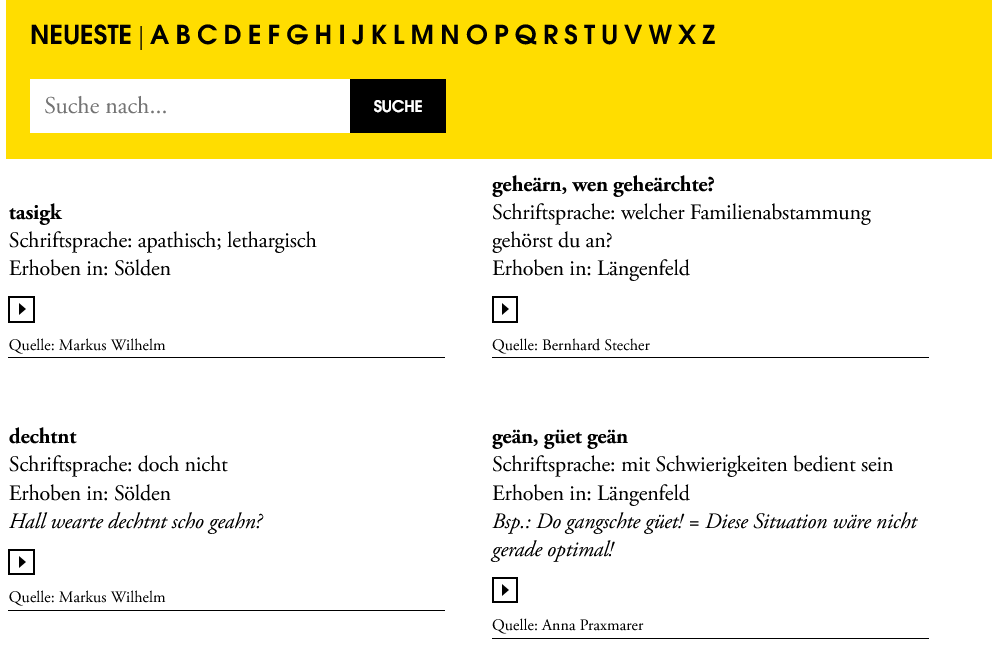
\includegraphics[width=\textwidth]{KathreinLaydialectcollectionsrevised-img007.png}
\caption{\label{fig:kathrein:7}The Ötztal collection is arranged in blocks and offers additional audio material as well as the source, sometimes also the word in its syntactic embedding.}
\end{figure}

The website states that the aim of the joint collecting project is to raise awareness of language in general and of the peculiarities of the Ötztal dialect and to appreciate both one’s own identity and that of other regions. In this respect, the purpose of the collection can be seen as raising (regional) linguistic awareness and thereby achieving a comprehensive appreciation of all identities.
%\enlargethispage{\baselineskip}
The intention of the original collectors is not known to us. Indirectly, however, the purpose of documentation is also addressed when “personalities involved in the documentation of Ötztal \emph{peculiarities} [emphasis by author]”\footnote{Original: “[…] auch zahlreiche weitere um die Dokumentation der Ötztaler Besonderheiten bemühte Persönlichkeiten […]” (\url{http://oetztalermuseen.at/forschung/oetztaler-dialekt-woerterbuch/}) (Accessed December 31, 2022)} are mentioned on the website, whose collections have been integrated into the overall collection.

\subsubsection{The Waidring collection}
\label{sec:kathrein:3.1.3}
The dialects of the so called “Tiroler Unterland” (see \figref{fig:kathrein:4}), i.e. especially those east of the area around Schwaz, are assigned to the Middle Bavarian transition area (see \figref{fig:kathrein:5}). Among the characteristics are the vocalization of postvocalic \textit{l} (dial. /hoits/ vs. Southern Bavarian /holts/ ‘wood’, dial. /vɔyt/ vs. Southern Bavarian /vɛlt/ ‘world’, dial. /muix/ vs. Southern Bavarian /milx/ ‘milk’), the lenition of intervocalic \textit{t} (dial. /veːdɐ/ vs. Southern Bavarian /ve̞tɐ/ ‘weather’) and the realization of mhg. \textit{ê} as a monophthong (dial. /ʃneː/ vs. Southern Bavarian /ʃneɐ/) ‘snow’). Another characteristic, but not limited to Middle Bavarian, is the fricative realization of \textit{r} before dentals as in \textit{Bart} (dial. /bɔːʃt/ ‘beard’) or \textit{Herz} (dial. /hɛɐʃts/ ‘heart’) (cf. \citealt[125]{Kranzmayer1956}, §50e3). 

\begin{table}
\begin{tabular}{lllll}
\lsptoprule
{mhg.} & {mhg. example} & {Waidring} & {example from collection} & Southern\\
& & & & Bavarian \\
\midrule
{V\textit{{}-l}} & \textit{h}\textbf{\textit{ol}}\textit{z} & /oi/ & /h\textbf{oi}ts/ ‘wood’ & /ol/\\
& \textit{w}\textbf{\textit{ël}}\textit{t}
& /ɔy/& /v\textbf{ɔy}t/ ‘world’ & /ɛl/ \\
& \textit{m}\textbf{\textit{il}}\textit{ch} & /ui/ & /m\textbf{ui}x/ ‘milk’ & /il/\\
\midrule
{ V-\textit{t}{}-V} & \textit{wë}\textbf{\textit{t}}\textit{er} & /d/ & /veː\textbf{d}ɐ/ ‘weather’ & /t/\\
\midrule
\textit{ê} & \textit{sn}\textbf{\textit{ê}} & /eː/ & /ʃn\textbf{eː}/ ‘snow’ & /ɛɐ/\\
\midrule
\textit{{}-rt-} & \textit{ba}\textbf{\textit{rt}} & /ʃt/ & /bɔː\textbf{ʃt}/ ‘beard’ & /rt/ \\
\textit{{}-rz-} & \textit{hë}\textbf{\textit{rz}}\textit{e} & /ʃts/ & /hɛɐ\textbf{ʃts}/ ‘heart’ & /rts/\\
\lspbottomrule
\end{tabular}
\caption{\label{tab:kathrein:3} Some of the characteristics of the Middle Bavarian dialect of Waidring as opposed to Southern Bavarian dialects}
\end{table}

For the eastern part of the country, a collection supported by a dialect association called “Insa Tirola Mundart” was selected. Here, too, already existing collections were combined into an online collection (\url{https://www.tiroler-mundart.at/woos-moast}) representing the northeasternmost part of the so-called Tiroler Unterland (see \figref{fig:kathrein:4}). However, since the collections are based on dialects that differ more from each other in some respects than in the other two regions, a partial collection was selected from them that concerns the community of Waidring. It was created by a member of the association for his home village and contained 2949 entries at the time of the material extraction on April 12, 2021. It is arranged in columns and provides additional audio material that embeds the entry in a syntactic context. The audio file for the entry \textit{Grieß} e.g. informs about the following: [ums go͜ed is vidɐramo͜e a vyːds kriːs] [‘Once again, there is a rather heated dispute over the money.’; author’s translation]. Thus, the translation of \textit{Grieß} as “starke Nachfrage” (‘strong demand’) is supplemented by the additional syntactic embedding in the audio file. Here, too, the search works both via an alphabetical bar and via text input, searching the columns “Mundart” as well as “Hochdeutsch” (see \figref{fig:kathrein:8}). Sometimes there are pictures linked to it that visually support the entry.

  
\begin{figure}
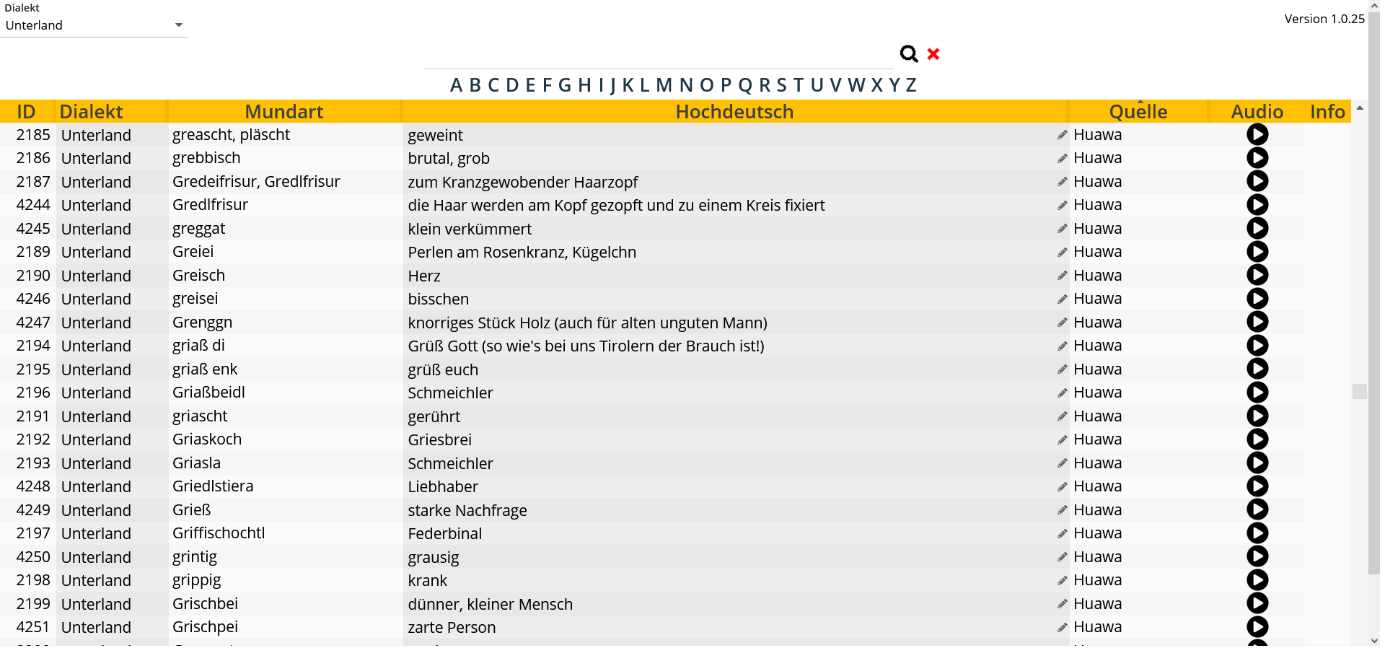
\includegraphics[width=\textwidth]{KathreinLaydialectcollectionsrevised-img008.png}
\caption{The collection from Waidring was created by a collector who is called “Huawa”; it is integrated into a larger collection.}
\label{fig:kathrein:8}
\end{figure}

The purpose is similar to the one from the Paznaun valley: the provision of a reference work\footnote{“Die Intention ist, möglichst viele Mundartliebhaber zu animieren, Mundartbegriffe aber auch fertige Wörterbücher zu integrieren, um eine umfassende Datenbank anbieten zu können.“ [‘The intention is to encourage as many dialect lovers as possible to integrate dialect terms but also dictionaries in order to offer a comprehensive database.’; author’s translation] (\url{https://www.tiroler-mundart.at/woos-moast/})} and the preservation of local dialects.\footnote{``Wir sehen es als unsere Aufgabe, die Mundart durch Digitalisierung einerseits einfacher zu verstehen (sehen, hören statt lesen) und andererseits in die Zukunft mitzunehmen.'' [‘We see it as our task, on the one hand, to make the dialect more understandable through digitalization (see, hear instead of read) and, on the other hand, to lead it into the future.’; author’s translation] (\url{https://www.tiroler-mundart.at/})}  Unlike the Paznaun collection, it is clear here that the association also wants to contribute to the continuity of the dialects.\footnote{“Wir […] wollen den Erhalt und die Pflege der Mundart des Tiroler Unterlands fördern.“ [‘We [...] want to promote the preservation and cultivation of the dialect of the Tyrolean lowlands.’; author’s translation] (\url{https://www.tiroler-mundart.at/}) „Du wüst ins hoifen, das ma insa Mundart pflegen und fie die Zukunft dahoit'n?“ [`You want to help us maintain our dialect and preserve it for the future?'; author’s translation] (\url{https://www.tiroler-mundart.at/mitglied-insa-tiroler-mundart/})}

What unites the three collections, then, is their similar purpose. This puts them in line with very many other collections, as Baur explains:

\begin{quote}
\foreignlanguage{ngerman}{%
Die in ihrem Bestand als gefährdet angesehene Mundart soll für spätere Generationen […] dokumentiert und vor dem Vergessen bewahrt werden. Darüber hinaus wollen nicht wenige durch ihre Sammelarbeit die Mundart pflegen, sie konservieren und ihr neue Freunde, Sprecher und Leser, zuführen. Immer öfter wird in Vorworten der Dialekt als ein wichtiger Bestandteil örtlicher oder regionaler Kultur bezeichnet, den es zu erhalten gilt. Mundartwörterbücher sind also als ein Mittel, lokale Identität zu erhalten oder wiederzugewinnen.}\footnote{‘The dialect, which is considered endangered in its existence, should be documented for later generations [...] and saved from oblivion. In addition, quite a few want to maintain the dialect through their collecting work, to preserve it and to bring it new friends, speakers and readers. More and more often the dialect is described in prefaces as an important component of local or regional culture, which must be preserved. Dialect dictionaries are therefore a means of preserving or regaining local identity.’ [author’s translation]} \citep[53]{Baur1987}
\end{quote}

\subsection{Sampling}
\label{sec:kathrein:3.2}
The samples for the Paznaun and Ötztal collection were taken on August 2, 2021, and those for Waidring on April 12, 2021. Due to the size of the collections, 70 randomly selected entries were taken for each collection, resulting in a total of 210 lemmas/syntagmas to be analyzed. However, for two collections, parts of it were already excluded in advance:

Due to a cooperation project with the Tyrolean Dialect Archive of the University of Innsbruck, the dialect documents of the scientist Eugen Gabriel had been integrated into the Ötztal collection. Of course, these are not amateur documents, which is why they were excluded from the sampling.

As already mentioned, only the partial collection of the collector “Huawa” from Waidring was selected as a sample for the collection of the “Tiroler Unterland”. I therefore call it the Waidring collection.

\subsection{Documentation of deviations}
\label{sec:kathrein:3.3}
All 210 entries were then cross-referenced with the Austrian dictionary (cf. \citealt{PabstEybl2018}), the German variant dictionary (cf. \citealt{AmmonEtAl2016}), the \textit{DWDS} (Digitales Wörterbuch der deutschen Sprache) and \textit{Duden online} \citep{DudenOnline}. This means that, on the one hand, lexical and semantic deviations from both the Federal German (viz. German standard language associated with Germany) and the Austrian standard language were documented. On the other hand, phonological and morphological deviations were documented and subsequently subjected to a phonological distance measurement according to Levenshtein (see \sectref{sec:kathrein:5.2}). In addition, register, style, and age information, as well as the approximate diatopic distribution of each item, were recorded if the dictionaries provided information about that.

\section{Questions and hypotheses}
\label{sec:kathrein:3.4}
As stated in \sectref{sec:kathrein:1}, I consider lay dialect collections as a source for perceptual dialectology, since their contents indirectly shed light on what lay people consider their dialect. Presumably, the items prototypically represent those words or phrases, that are salient to them, that best characterize their dialect, that make it up.

This study therefore focuses on the following two questions: 

\begin{itemize}
\item What do laypersons’ dialect collections contain? 
\item How “dialectal” are the collections, i.e. where on the dialect standard axis are the items located? 
\end{itemize}

\begin{sloppypar}
“Dialekte sind die standardfernsten, lokal oder kleinregional verbreiteten Voll-varietäten.” \citep[59]{SchmidtHerrgen2011} Bearing in mind this definition of \citet{SchmidtHerrgen2011} according to which dialects are~– among other things~– furthest from the standard, I assume that 
\end{sloppypar}

\begin{enumerate}
\item dialect collections created by laypersons contain mostly items that do not exist in the standard language.
\end{enumerate}

Apart from the collectors’ intention to record words that are in the process of being forgotten, this assumption is supported by Baur’s observation that it is often “conspicuous, inexplicable or particularly old words” (\citealt[66]{Baur1987}; author’s translation) that are considered worth recording. Such words are hardly words of the standard language, but dialect words.
\largerpage[-2]

The peculiarities of a dialect which are also to be transported in such collections can find their expression not only on the lexematic, but also on the phonological and/or morphological level. Therefore, I further assume that

\begin{enumerate}[resume] 
\item if the items do exist in the standard language, they 
\begin{itemize}
\item[a)] have a considerable phonological and/or morphological distance and/or
\item[b)] are semantically distinguished from its equivalent in the standard language.
\end{itemize}
\end{enumerate}

\section{Results}
\label{sec:kathrein:5}
\subsection{Deviations on the linguistic levels}
\label{sec:kathrein:5.1}
In keeping with the purpose of the collections described in Sections~\ref{sec:kathrein:3.1.1}--\ref{sec:kathrein:3.1.3}, I expect to find a relatively large number of words and/or phrases that demonstrate the distinctive features of the dialect in question; that is, I expect to find words that have no equivalent in the standard language either because of differences at the lexematic or semantic level.

It must be added that some words, of course, vary not only on one linguistic level, but on several. For example, the dialectal word \textit{Gschlatter} is contrasted with its equivalent \textit{Gschlader} [ˈkʃlaːdɐ], which is marked as colloquial but can be found in the standard dictionary. The dialectal word refers to a semi-liquid mass (dough, mortar) that is (deliberately) sloppily mixed together\footnote{‘(oft absichtlich) schlampig zusammengerührte halbflüssige Masse (Teig, Mörtel)‘} whereas the “standard” word refers to an inferior drink, a thin coffee\footnote{‘minderwertiges Getränk, dünner Kaffee‘}. Therefore, on the one hand, they differ in their semantics. In addition, the dialectal word is realized with a fortis plosive ([ˈkʃlatr]), while the “standard” word is realized with a lenis plosive [ˈkʃlaːdɐ]. Thus, they also differ at the phonological level. This leads to the classification as “phon-sem” (another example of a phonological, morphological and semantic deviation is \textit{Plot} in \tabref{tab:kathrein:5b}).


\subsubsection{Lexical and semantic deviations}
\label{sec:kathrein:5.1.1}

\tabref{tab:kathrein:4} shows the percentages of deviant elements on the different linguistic levels for all three samples. As can bee seen, words that do not exist in the standard language or that exist but differ on a semantic level make up about half of the sample (53 \% Paznaun, 57 \% Ötztal, 50 \% Waidring).


\begin{table}
\begin{tabularx}{.8\textwidth}{Qrrr}
\lsptoprule
& \textit{Paznaun} & \textit{Ötztal} & \textit{Waidring} \\
\midrule
\textbf{lex} & \textbf{46} & \textbf{49} & \textbf{37} \\
%\cmidrule{--~-~-~}
\textbf{only sem} & \textbf{-} &  \textbf{4} &  \textbf{6} \\
%\cmidrule{--~-~-~}
\textbf{phon-sem} & \textbf{4} & \textbf{4} &  \textbf{6} \\
%\cmidrule{--~-~-~}
\textbf{phon-morph-sem} & \textbf{-} & \textbf{-} &  \textbf{1} \\
%\cmidrule{--~-~-~}
\textbf{morph-sem} & \textbf{3} & \textbf{-} & \textbf{-}\\
\textit{SUM} & \textbf{53} & \textbf{57} & \textbf{50}\\
\midrule
only phon & 33 & 23 & 29 \\
%\cmidrule{--~---~}
phon-morph & 10 & 14 & 11\\
%\cmidrule{--~---~}
phon-syn & 2 & 2 & -\\
%\cmidrule{--~---~}
only morph & 1 & 1 & 3 \\
% \cmidrule{--~---~}
no difference & 1 & 3 & 7\\
\textit{SUM} & 47 & 43 & 50 \\
\lspbottomrule
\end{tabularx}
\caption{\label{tab:kathrein:4} Linguistic-levels-profile of the three samples. In the Paznaun sample, 53 percent have no lexical equivalent or different semantics, in the Ötztal sample it is 57 percent, in the Waidring sample 50 percent (all in bold letters).}
\end{table}

Which words make up this half? As far as the lexical level is concerned, there are words like \textit{ånlag} (Paznaun) ‘comfortable, even (to walk)’, \textit{vrkåltn} (Ötztal) ‘to put away’, \textit{Schüehenooch} (Ötztal) ‘kick’ or \textit{Kartoffelwiala} (Waidring) ‘dish from steamed potatoes’. In this case, either the object/concept does exist in both systems but is realized in completely different ways (\textit{ånlag}, \textit{vrkåltn, Schüehenooch}) or the word refers to an object that is only locally common and has therefore no equivalent in Standard German (\textit{Kartoffelwiala}; see \tabref{tab:kathrein:5a}).

Semantic differences, on the other hand, can be seen, for example, in the word \textit{Muli}: There does exist the word \textit{Muli} in Standard German, but it neither means `donkey' nor `drunkenness' as the dialect word suggests. It just means `mule' in Standard German, which is a crossing between donkey and horse. Of course, other linguistic levels may be involved here, as outlined above; nevertheless, the semantic difference remains the most important for classification. This applies, for example, to the word \textit{Plot}, which is pronounced [plɔt] in the local dialect\footnote{Weak feminina are subject to the e-syncope in Middle Bavarian \citep[K. 57]{KleinEtAl1965}}, while in Standard Austrian it is [plate̞] (see \tabref{tab:kathrein:5b}).

\begin{sidewaystable}
\caption{Items that differ on a lexical level}
\label{tab:kathrein:5a}
\footnotesize
\begin{tabularx}{\textwidth}{ l >{\raggedright}p{4cm} cQ }
\lsptoprule
&         &   standard &  \\
&         &  equivalent & entry in dialects dictionaries \\\midrule
\multicolumn{4}{l}{\textit{ånlag} (Paznaun) }\\
& ‘bequem, eben (zu gehen)’ (‘comfortable, flat (to walk)’) & - & yes, but narrower range of meanings: ‘vom Gelände, leicht ansteigend, wenig geneigt’ (‘slightly ascending terrain, little inclined’; \citealt[19]{Schatz1993})\\
\multicolumn{4}{l}{\textit{vrkåltn} (Ötztal)}\\
& ‘verräumen’ (‘to put away’) & - & no, merely \textit{aukąltn} `aufbewahren‘ (`to store sth.’; \citealt[276]{Schatz1993}) and  \textit{g(e)halte\textsuperscript{n}} `etw. in ein Behältniss legen, an seinem gehörigen Ort, Versteck aufheben, im Stand erhalten, eig. und bildl.' (‘to put something in a container, to keep in its proper place/hiding place, to keep in state, proper and figurative’; \citealt[1235]{StaubEtAl1885}) \\
\multicolumn{4}{l}{\textit{Schüehenooch} (Ötztal)}\\
& `Fußtritt' (‘kick’, literally ‘foot kick’) & - & no, only noun \textit{fuɛssiną̂rsch} (literally `foot in the ass'; \citealt[193]{Schatz1993}) and verb \textit{fuessârsche} `giving kicks in the bottom with your ass' (\citealt[467]{StaubEtAl1885})\\
\multicolumn{4}{l}{\textit{Kartoffelwiala} (Waidring)}\\
& `geriebene Erdäpfel gedünstet' (`dish from steamed potatoes') & - & yes (WBÖ-Database\footnote{\url{https://lioe.dioe.at/db}, accessed October 10, 2023.} entry \textit{Wirler}, nr. 1C.2a29)\\
\lspbottomrule
\end{tabularx}
\end{sidewaystable}

\begin{sidewaystable}
\footnotesize
\caption{Items that differ on a semantic level}
\label{tab:kathrein:5b} 
\begin{tabularx}{\textwidth}{ l >{\raggedright}p{4cm} QQ }
\lsptoprule
&  & standard  & \\
&  & {equivalent} & entry in dialects dictionaries \\
\midrule

\multicolumn{4}{l}{\textit{Muli} (Waidring)}\\
& `Esel, Rausch' (`donkey', `drunkenness') & \textit{Muli} `Maultier' (`mule') & yes, but only in parts of South Tyrol (\citealt[437]{Schatz1993})\\
\multicolumn{4}{l}{\textit{Plot} (f.) [plɔt] (Waidring)\footnote{\textit{Plot} additionally differs on phonological and morphological level.}}\\
& `Schulter' (`shoulder') & \textit{Platte} [plate̞] among others `verschiedenen Zwecken dienendes flaches Stück aus einem bestimmten Material, dessen Dicke im Verhältnis zu den anderen Abmessungen gering ist'
(`flat piece of a certain material serving various purposes, the thickness of which is small in relation to the other dimensions') & no\\
\lspbottomrule
\end{tabularx}
\end{sidewaystable}

This half (words non-existent in the standard with different semantics) forms, so to speak, what could be understood as a dialect collection in the narrowest sense: It consists of words which are completely excluded from standard dictionaries or which differ semantically from entries in standard dictionaries.

A look at the dialect dictionaries compiled by scholars, on the other hand, reveals interesting aspects (see \tabref{tab:kathrein:5a}). First, some of the words collected by laymen (\textit{vrkåltn}, \textit{Schüehenooch}, \textit{Plot}) are not listed in them at all, which is probably because the question books on which the dictionaries are (coincidentally) based did not aim to do so (or else because the “question book makers” simply did not think to query them). Second, some words are listed, but not semantically differentiated in such a way that the local meanings emerging from the lay collections could have been taken into account (\textit{ånlag}, \textit{Muli}).\largerpage[2.25]

This small finding already shows how fruitful the inclusion of such lay collections would be in the compilation of dialect dictionaries, not only to have questionnaires created by scientists answered by lay people, but also to enrich the dictionary with introspectively generated lay data and thus come closer to the language reality.\footnote{In a sense, the work of scientists is also introspection, since they, too, map only a part of reality through the creation of their questionnaires, albeit a very well-founded one. \citet{HoferMeier2015} speak here of the fact that lexicographical competence and, in particular, the introspection of dictionary makers alone are actually not sufficient for scientific purposes to represent language in its natural environment: “Die Lexikographenkompetenz allein ist für einen Intersubjektivität anstrebenden wissenschaftlichen Standard jedoch ungenügend, denn durch allzu starke introspektive Ausrichtung [der WörterbuchmacherInnen, YK] wird der eigentliche Untersuchungsgegenstand – die Sprache in ihrem natürlichen Umfeld – verfehlt.” \citep[120]{HoferMeier2015}} Since these lay collections were often created by several authors in joint consultation, the material can certainly be considered reliable. Combining this with an online survey to verify entries would provide additional reliability (cf. \citealt{HoferMeier2015}, \citealt{Retti1999}). And it is a starting point to re-examine the question of subjective and objective data that has preoccupied perceptual dialectology since its inception: To what extent can subjective data on the dialect perception of laypersons (perception data) be reconciled with production data determined objectively by scientists? When is reconciliation being canceled? And why? (cf. \citealt{Preston1999}) Applied to our collections, this would mean: What words have been introspectively included in a lay collection that do not appear in a dialect dictionary produced by scientists? And why? Is it because of the recording method? Or are individual entries too widespread and/or too close to the standard to be included in a dialect dictionary? Are the lay collectors not even aware of this and do such words belong to their understanding of dialect, which would then be very broad? Or are they aware of this and include such words in their collections anyway because they are used in everyday speech, no matter how base dialectal they are? To explore this is beyond the scope of this article. Qualitative interviews with lay collectors would be additionally necessary to shed light on these questions.{\interfootnotelinepenalty=10000\footnote{A first pilot interview in this context has already shown, for example, that laypersons are quite capable of observing language closely and that they are quite aware that there are gaps in the material. However, it also became clear that a lot of things happen unconsciously.}}

\subsubsection{Phonological and morphological deviations from the standard language}
\label{sec:kathrein:5.1.2}
As far as the other half is concerned, it consists of deviations that only occur on the phonological or morphological level or it is a combination of both (see \tabref{tab:kathrein:4}). Of course they follow the sound laws of the respective dialects: It is words like \textit{brat} [braːt] vs. \textit{breit} [brait] (= ‘broad, wide’) in the Paznaun sample, \textit{Viich} [viːç] vs. \textit{Vieh} [viː] (= ‘animal, livestock’) in the Ötztal sample or \textit{heazoagn} [ˈhɛɐtsɔɐŋ] vs. \textit{herzeigen} [ˈhɛɐtsaigŋ] (= ‘to show’) in the Waidring sample. Given its relative closeness to the standard variant, its occurrence in a dialect collection may be surprising. However, at least in the Paznaun sample, 21 out of 33 (= 63 percent) of this second half are marked either in terms of regional distribution (e.g. Austria and/or Southern Germany), style (colloquial, slang, elevated) or the age of the word (archaisms). Thus, words such as \textit{flattiara} or \textit{Dolba} make up about two thirds of those words only deviating on a phonological and/or morphological level (see \tabref{tab:kathrein:6}).


For the Waidring and the Ötztal sample, this is slightly different: Stylistically marked words such as \textit{potzn} ‘to blot’ in Waidring make up 49 percent (= 17 out of 35) whereas in Ötztal words such as \textit{tochtlen} ‘to slap someone (across the face)’ only make up 19 percent (= 6 out of 31).

\begin{table}[h]
\begin{tabularx}{\textwidth}{QQQY}
\lsptoprule
 {dial.} & {std.} & {meaning} & {percentage of marked items}\\
 \midrule
\multicolumn{4}{c}{\bfseries Paznaun}\\
\midrule \textit{flattiara} & \textit{flattieren}
used in Switzerland, archaic in Austria and Germany & ‘to flatter someone' & 63\\
\cmidrule{1-3}
\textit{Dolba} & \textit{Dolm}
Austrian, colloquial, offensive & ‘stupid person' & \\
\midrule
\multicolumn{4}{c}{\bfseries Waidring}\\
\midrule
\textit{potzn} & \textit{patzen}
Bavarian, Austrian & ‘to blot’ & 49\\
\midrule
\multicolumn{4}{c}{\bfseries Ötztal}\\
\midrule
\textit{tochtlen} & \textit{dachteln}
East Middle German, Southern German, Austrian, colloquial & ‘to slap someone (across the face)’ & 19\\
\lspbottomrule
\end{tabularx}
\caption{\label{tab:kathrein:6} Examples of items that a) only differ on a phonological and/or morphological level and that b) are marked somehow.}
\end{table}

There are even a few items (7, 3 and 1 percent) that show no difference – at least no phonological difference – to the standard variant at all. However, such items are again mostly words that are marked either as colloquial or as slang or that only show a certain regional or functional distribution. The only visible difference is that they sometimes differ in terms of graphemes (see \tabref{tab:kathrein:7}).

\begin{table}
\begin{tabularx}{\textwidth}{QQQY}
\lsptoprule
 {dial.} & {std.} & {meaning} & {percentage of items not differing}\\
\midrule
\multicolumn{4}{c}{\bfseries Waidring}\\
\midrule
\textit{Zwiesl} & \textit{Zwiesel}
local & ‘tree with forked trunk and two crowns’ & 7\\
\cmidrule{1-3}
\textit{wist} & \textit{wist} & ‘Haw!’ [command to a horse to turn to the left] & \\
\cmidrule{1-3}
\textit{Häfn}, \textit{Hefn} & \textit{Häfen}
Austrian, colloquial & among other things: ‘prison’ & \\
\cmidrule{1-3}
\textit{sinnian} & \textit{sinnieren}
colloquial & ‘to ponder‘ & \\
\cmidrule{1-3}
\textit{Hanni} & \textit{Hanni} & ‘female surname’  (Johanna) & \\
\midrule
\multicolumn{4}{c}{\bfseries Ötztal}\\
\midrule
\textit{Murgs} & \textit{Murks}
colloquial, pejorative, casually & ‘sloppy, poor work’ & 3\\
\cmidrule{1-3}
\textit{Scheniiror} & \textit{Genierer}
colloquial, esp. Austrian & ‘shame’ & \\
\midrule
\multicolumn{4}{c}{\bfseries Paznaun}\\
\midrule
\textit{drinn} & \textit{drin}
colloquial & ‘inside’ & 1\\
\lspbottomrule
\end{tabularx}
\caption{\label{tab:kathrein:7} All items of the samples that phonologically and/or morphologically do not differ from its standard equivalent.}
\end{table}

So, on the one hand, we can observe that about half of the items in our samples deviate lexically or semantically from standard language. Whether the first hypothesis (“dialect collections created by laypersons contain mostly items that do not exist in the standard language”) as well as the second part of the second hypothesis (“if the items do exist in the standard language they are semantically distinguished from its equivalent in the standard language”) can be confirmed by this might depend on what is meant by “mostly”: If by this is meant “more than half”, it can be said for at least two of the three samples that they consist mainly of words not found in the standard language. However, given the small number of items examined, this result can only be an approximation and we can state: It seems that words not found in the standard language are an important part of the dialect collections of laypeople.

The other half consists of words that differ on the phonologial and/or morphological level, with a certain number of words marked (Paznaun about two thirds, Ötztal about half, Waidring one fifth). In this, the samples differ considerably. Interestingly, there is a small percentage of words that do not differ from the standard pronunciation. But, again, almost all of these items are marked stylistically. To test the first part of the second hypothesis (“if the items exist in the standard language, they have a considerable phonological and/or morphological distance”), the deviations on these two levels have to be measured, which will be described in the next chapter.

\subsection{Measuring phonological and morphological deviations}
\label{sec:kathrein:5.2}
Here we now want to pursue the question of how much the items deviate phonologically and morphologically from Standard German. Thus, we are concerned with the degree of dialectality of each item, i.e., the phonetic distance between an individual dialect word and its standard counterpart, which is indicated by the $d$-value (short for dialectality value).

For this purpose, each word was subjected to a normalized dialectality measurement according to Levenshtein (cf. \citealt{Heeringa2004}).\footnote{These calculations were performed using Peter Kleiweg’s online tool: \url{https://urd2.let.rug.nl/~kleiweg/L04/webapp/bin/home} (accessed on December 26, 2022). The Levenshtein distance was preferred to the method developed by Herrgen/Schmidt (cf. \citealt{HerrgenSchmidt1989}, \citealt{Lameli2004}), which is otherwise widely used in variational linguistics, for the simple reason that it provides an automation-based tool that allows for rapid measurements. Nevertheless, the Levenshtein distance measurement is also used in variational linguistics, especially in the Dutch area (cf. \citealt{GooskensHeeringa2004}; a compilation of different methods can be found in \citealt{NerbonneHeeringa2009}). Levenshtein also proves to be advantageous in evaluating other collections, since audio material is not always available, but one must infer pronunciation from the mere spelling of the items.} That is, the individual items (in our case, the sounds) of one “chain” (in our case, the phonetically transcribed words) are compared with those of another chain. The goal is to calculate how many transformations must be made to the individual sounds in order to move from one chain to another. This is done by taking away, adding or substituting elements. However, each of these transformations “costs” something. The sum of the costs then gives the $d$-value. For example, it is calculated how much it costs to get from the dialect pronunciation [glandɐ] to the Standard German pronunciation [ge̞lɛndɐ] (‘railing’).

\begin{table}
\begin{tabular}{cccccccc}
\lsptoprule
1 & 2 & 3 & 4 & 5 & 6 & 7 & \\
g &  & l & a & n & d & ɐ & \\
g & e̞ & l & ɛ & n & d & ɐ & \\
\midrule
& 1 &  & 1 &  &  &  & 2\\
\lspbottomrule
\end{tabular}
\caption{\label{tab:kathrein:8} Measuring Levenshtein distance}
\end{table}

Each operation here costs 1\footnote{A vowel-consonant substitution even costs 2, thus ʃiɐ vs. ʃøːn (‘nice’) would be 1 + 2 = 3.}, which then gives a value of 2. To include the length of the word in the calculation, the value was normalized, which means that the result was divided by the number of alignment slots (2 ÷ 7 = 0.29). Thus, the $d$-value of [glandɐ] compared to [ge̞lɛndɐ] is 0.29. (cf. \citealt{BeijeringEtAl2008}) This means that a little less than one third of the word shows deviations from the standard language.

For the calculations of the $d$-values, all words in question were broadly transcribed on the basis of the available audio files or on the basis of my own dialect competence (see \sectref{sec:kathrein:3.1.1}). They have been transcribed broadly since I assume that allophones such as [x] {\textasciitilde} [ç], [ʀ] {\textasciitilde} [r], [ɐ] {\textasciitilde} [ə] are not conscious to laypersons or that these sounds are not the reason for inclusion in a collection. Standard Austrian pronunciation served as a basis for comparison, differing from Standard German pronunciation primarily in that /s/ is unvoiced in a vowel environment (e.g., Austrian /saːgŋ/ vs. Federal German /zaːgŋ/), short /i/ and /y/ are not centralized (e.g. Austrian /milç/, /glyk/ vs. Federal German /mɪlç/, /glʏk/) and short final /e/ or those occurring in unstressed syllables are pronounced as /e̞/ rather than /ə/ (cf. \citealt{Wiesinger2009}). The words were generally transcribed in the allegro form (/maxn̩/ vs. /maxən/).

\figref{fig:kathrein:12} shows the $d$-values of phonologically and/or morphologically deviating items of the three samples. The medians (marked by a line) of the Paznaun and Ötztal samples are 0.5 (with average values of 0.45 and 0.46 resp., marked by an x), while the median of the Waidring sample is lower at 0.29 (average 0.34). This is consistent with the percentage of non-divergent elements (7 percent) and the lowest percentage of elements without a standard equivalent (50 percent, both see \tabref{tab:kathrein:4}): The Waidring sample seems to be less dialectal than the other two collections.

\begin{figure}
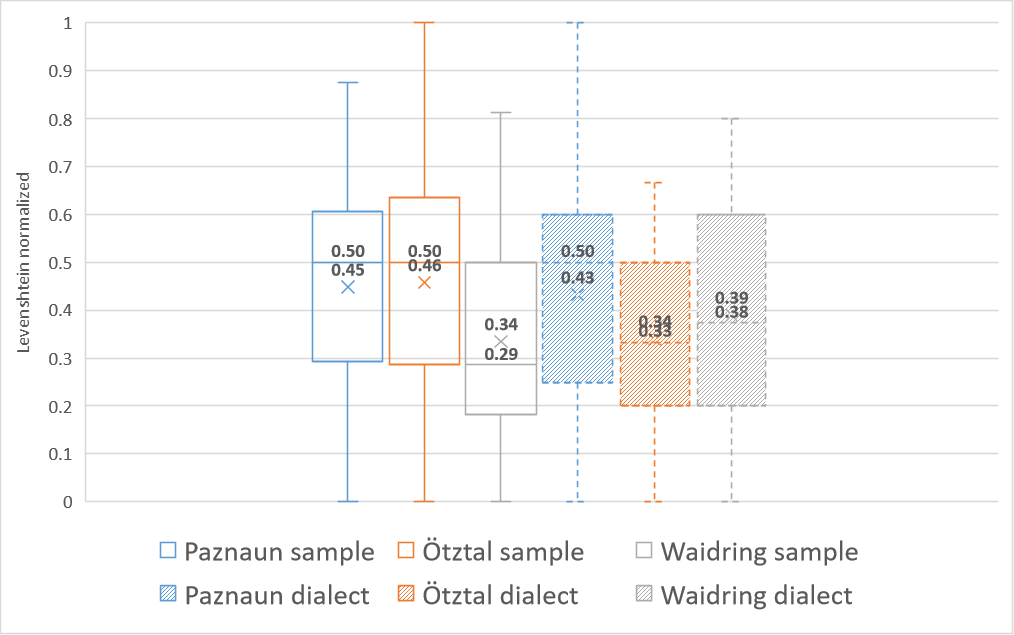
\includegraphics[width=\textwidth]{KathreinLaydialectcollectionsrevised-img012.png}
\caption{\label{fig:kathrein:12} Normalized dialectality values of the samples (left half of the figure; Paznaun: n = 33, Ötztal: n = 30, Waidring: n = 35) and of the underlying dialect (right half; n = 51 each).} 
\end{figure}

In order to rule out the possibility that it is not the dialect itself which has a lower degree of dialectality compared to the standard language, the $d$-value of the underlying dialect was also measured. For this purpose, the Wenker sheets available for the respective areas\footnote{The Wenker sheets are easily accessible via the REDE tool \url{https://apps.dsa.info/wenker/}. (Accessed August 08, 2024)} were evaluated, since they allow a good comparison due to the uniform template. For the Paznaun valley, Ischgl was chosen as the reference corpus, for Ötztal it was Sölden. For Waidring, of course, it remained Waidring. The words used for comparison have not changed significantly since the 1930s (i.e. since the time of recording). If they changed or a different lexeme was used, an alternative word from the holdings of the Tyrolean Dialect Archive was used for comparison for all three places.

Since the vowel system of the underlying dialects deviates more from the norm than the consonant system, each Middle High German vowel was assigned a reference word from the Wenker sentences. Phonetic contexts with nasals and liquids were also considered (e.g. mhg. \textit{{}-ân-} or mhg. \textit{{}-ër-}). In the consonantal domain, Middle High German \textit{t} (in intervocalic use) and \textit{l} (in postvocalic use) were used. This is because South Central Bavarian (to which the dialect in Waidring belongs) is especially characterized by vocalization processes. (see \sectref{sec:kathrein:3.1.3})

This selection inevitably simplifies the linguistic reality. To mitigate this effect, the comparison was not made between individual vowels and consonants in isolation, but rather between entire words. These words were chosen specifically for their reference sounds in Middle High German. In addition, further phenomena (e.g. morphological) come into play (final -\textit{en}, prefix \textit{ge}{}- for participles, \textit{n}{}-apocope, \textit{e}{}-apocope for weak feminines, etc.). Examples of this comparison are shown in \tabref{tab:kathrein:9} (for the complete list see \sectref{sec:kathrein:appendix}: Appendix).

\begin{table}
\begin{tabular}{lllllc}
\lsptoprule
 & {mhg.}  & {word} & {dial.} & {std.} & {$d$}\\
 \midrule
Ischgl &  &  & saːfɐ & & 0.50\\
Sölden & ei/-e (fem.) & S\textbf{ei}f\textbf{e} & sɔɐfe̞ & saife̞ & 0.40\\
Waidring &  &  & sɔɐf &  & 0.60\\
\midrule
Ischgl & & & gloubɐ & & 0.50\\
Sölden & ou/-en & gl\textbf{au}b\textbf{en} & glɵːbm & glaubm & 0.33\\
Waidring &  &  & glaːm &  & 0.42\\
\midrule
Ischgl & & & falt & & 0.25\\
Sölden & ël & F\textbf{el}d & falt & fɛlt & 0.25\\
Waidring &  &  & føit &  & 0.75\\
\midrule
Ischgl & & & toː & & 0.80\\
Sölden & ge-t/ân  & \textbf{getan} & ge̞tɔːn &   ge̞taːn & 0.20\\
Waidring &  &  & tũː &  & 0.67\\
\midrule
Ischgl &  &  & milx &  & 0.00\\
Sölden & il & M\textbf{il}ch & milx & milx & 0.00\\
Waidring &  &  & muix &  & 0.50\\
\midrule
Ischgl &  & & ʃiɐ &  & 1.00\\
Sölden &  -œn/-n\footnote{after root vowel}& sch\textbf{ön} & ʃɛɐn & ʃøːn & 0.67\\
Waidring &  &  & ʃẽː &  & 0.67\\
\midrule
Ischgl &  & & birʃtɐ & & 0.50\\
Sölden & -rst-/-e (fem.) & Bü\textbf{rste} & biːxta & byrste̞ & 0.67\\
Waidring &  &  & biːʃt &  & 0.67\\
\lspbottomrule
\end{tabular}
\caption{\label{tab:kathrein:9} Examples of words from the Wenker material whose local pronunciation was compared to the Standard Austrian pronunciation. The column “mhg.” indicates which sound, sound combination or morpheme was targeted in the respective word.}
\end{table}

The results of the calculations can be seen on the right part of \figref{fig:kathrein:12} (dashed bars). This shows that the $d$-value for the dialect of the Paznaun valley corresponds closely with that of the sample (blue boxes; 0.5 medians, 0.45 vs. 0.43 average). Thus, the collectors seem to be able to represent their dialect quite well in the collection. Words that differ phonetically\slash morphologically from the standard are not overrepresented in the sense that they would exceed the $d$-value of the Wenker material (which might be expected in a collection that aims to document idiosyncrasies that need not be in the lexical domain alone).

This is the case for the Ötztal sample (orange boxes): Here, a median $d$-value of 0.5 (or 0.46 on average) for the sample contrasts with a median $d$-value of 0.33 (or 0.34 on average) for the underlying dialect. In this collection, too, the focus is on the special features of the Ötztal dialect; however, in contrast to the Paznaun valley, the Ötztal idiosyncrasies on the phonological and morphological level are strongly condensed in the single collected items. Words such as dial. \textit{Keer} [kxɛɐr] versus std. \textit{Gehör} [ge̞høɐ] ‘sense of hearing’ ($d$-value: 0.83) or dial. \textit{Gewåchsnr} [ge̞vɔksnr] versus std. \textit{Erwachsener} [ɛɐvaksnɐ] ‘adult’ ($d$-value: 0.75) will account for this.

The Waidring collection, on the other hand, seems to be less dialectal than it could have been in terms of phonological and morphological features. With a $d$-value of 0.29 (median; or 0.34 on average), the sample has the lowest degree of dialectality, as already noted. There, we find words such as \textit{vazochn} ‘ill-bred’ (dial. [fɐtsoːxŋ̩] vs. std. [fɐtsoːgŋ̩] = $d$-value of 0.11) or \textit{Ralweg} ‘bikeway’ (dial. [raːlveːk] vs. std. [raːdveːk] = $d$-value of 0.17). Relative to the $d$-value of the underlying dialect, which is 0.38 (median; or 0.39 on average), however, the result is somewhat relativized (gray boxes).

What does this mean with regard to the first part of the second hypothesis (``If the items do exist in the standard language, they have a considerable phonological and/or morphological distance.”)? We can state that the Ötztal sample has the highest degree of dialectality, compared to the degree of dialectality exhibited by the underlying dialect. The $d$-value of the sample is 17 (medians) or 12 (average) percentage points higher than the Wenker material, which is certainly not negligible. Possibly this has to do with the large number of collectors who were and are involved: The more people involved, the better they get to the heart of the matter (whereby “many cooks” could of course also “spoil the broth”). In addition, the institutional framework in which the collection is embedded could be effective here: The Ötztal museums do not only want to collect and convey knowledge, but also to conduct research.\footnote{\url{http://oetztalermuseen.at/uber-uns/} (Accessed December 29, 2022)}

In this context, however, more detailed information would be needed about the possible intervention of the final editors, who are scientists. But perhaps this also has to do with a sharpened sense of one’s own variety; the linguistic awareness and self-image of the Ötztalers may have been spurred on by the inclusion of the Ötztal dialect as an intangible cultural heritage in 2010.\footnote{\url{https://www.unesco.at/kultur/immaterielles-kulturerbe/oesterreichisches-verzeichnis/detail/article/oetztaler-mundart} (Accessed December 29, 2022)} This may also be reflected in the fact that the phonologically and/or morphologically deviating words are the least frequently marked (19 percent; see \tabref{tab:kathrein:6}). Thus, we can probably indeed speak of the degree of dialectality being considerable in the Ötztal sample, even if stylistic markings could be more frequent.

The other two samples do not have a higher $d$-value than the underlying dialect (we neglect the difference between 0.45 and 0.43 here), but they are still quite and relatively close to this value, respectively, which means that especially in the case of the Paznaun sample, with its high proportion of marked words (63 percent, see \tabref{tab:kathrein:6}), one can also speak of a fairly substantial phonological/morphological difference to the standard language (always taking into account the $d$-value of the underlying dialect, of course).

The sample from Waidring, with its 49 percent  of marked words (see \tabref{tab:kathrein:6}) and its somewhat lower $d$-value than the underlying dialect indicates, can probably still be called dialectal, if not to a considerable, at least to a respectable extent.

Of course, one should not overinterpret these numbers in view of the small samples. But they can show a certain tendency, which is also confirmed with a similarly high number of lexical and semantic deviations, as we have already seen. And they show that lay dialect collections have sufficient linguistic evaluation potential, for example, with regard to the ideas lay people have about the vertical dimension of their dialect.

\section{Conclusions and research perspectives}
\label{sec:kathrein:6}

The samples of lay dialect collections from Tyrol examined in the study, namely from Paznauntal, Ötztal, and Waidring, show a similar composition: About half of the respective material deviates from the standard language on a lexical and semantic level, i.e., this half forms the core of what can, among other things, be understood as dialect, namely the variety that has the greatest distance from the standard language. This half, therefore, will certainly do the most justice to those collectors who not only want to document the dialect, but also to save it from oblivion and perhaps even to make it fit for the future. The exact proportion of such individuals in the collections cannot be determined, as multiple people~-- and in the case of the Ötztal region, a particularly large number~-- were involved. But we know the intention of the editors of the collections, which in all three cases is to document the respective dialect with its peculiarities.

These peculiarities may be reflected not only at the lexical and semantic level, but also at the phonological and morphological level. This makes up the other half of the samples. In this, however, the three collections differ quite clearly: In the sample for Paznaun, almost two-thirds of phonologically/morphologically divergent words are marked in terms of distribution, style, or age. Moreover, these words have a mean $d$-value of 0.5, so the Paznaun sample is quite strongly dialectal after all. In Waidring, half of the phonologically/morphologically divergent words are marked. This is contrasted with the lowest $d$-value of 0.29 (with a $d$-value of 0.38 of the underlying dialect). Thus, this sample might be somewhat more dialectal. In the Ötztal sample, only one fifth of the phonologically/morphologically deviant words are marked. However, the $d$-value must also be taken into account here, which is highest in this sample with 0.5 relative to the $d$-value of the underlying dialect (0.33). This might “allow” to include more unmarked words in a collection. Thus, the Ötztal sample is also very dialectal overall and can thus reflect the specifics of the dialect well.

The study of lay dialect collections naturally raises many questions. Most importantly, it stimulates further research, since such collections have not been perceived as a possible source for perceptual dialectology so far:

Apart from the fact that the samples would obviously have to be enlarged in order to provide representative results, it is obvious to conduct comparative studies, for instance with collections that have a different intention, e.g. those that have been created in a tourist context. There, clichéd, obscure, exotic, hard-to-pronounce, or otherwise strange words and phrases are to be expected with disproportionate frequency, just as a study of auto-stereotypes and meta\hyp stereotypes (= supposed auto-stereotypes) would be worthwhile as a comparison, regardless of the intention with which a collection was created. Because what you believe others would not understand, find funny or know in a different context, you may be more likely to include in your collection than something that does not interest others because of its (supposed) information content. Presumably, attitudes towards one’s own or other people’s varieties also play a role in this context. In this respect, a comparison with collections from other (federal) states or dialect areas could also provide new insights into possible regional differences.

\begin{sloppypar}
Theoretical penetration is one thing, practical processing is another. Ultimately, the linguistic considerations of “why?” are just as much a guess, for example: Why are words included whose dialectal value is very low to non-existent?
\end{sloppypar}

This leads to the question of whether measuring $d$-value is an appropriate way of addressing these collections at all, and to answer the question “why?”. After all, a word like [braːt] 'broad' (compared to the standard word [bra͜it]) may indeed have a normalized $d$-value of 0.3 according to Levenshtein. However, this says nothing about how “dialectal” this difference appears to laypeople, especially considering how this word is realized in surrounding dialects. It also says nothing about what laypeople are even aware of.

Certainly, saliency and prototypicality studies should therefore complement such analyses in which the subjects are asked, among other things, how they characterize their dialect or what is special/typical about it compared to other dialects in their region/dialects in other regions, and also what connects it to others. This is also conceivable in the opposite direction, if informants were asked which given words best represent the subjects’ dialect. This also suggests experimental arrangements in which the participants are asked to write down dialect words from their own dialect that occur to them spontaneously and to comment on them additionally or to discuss with each other afterwards why they have included the word (cf. e.g. the Pilesort method in the DFG project “Der deutsche Sprachraum aus der Sicht linguistischer Laien” (‘The German language area from the point of view of linguistic laypersons’), in which the subjects were also asked about the motives for their sorting. There, the question of differentiation from other dialectal units also arose, but not on a vertical but on a horizontal level) (cf. \citealt[52--54]{Schröder2017}). Therefore, qualitative interviews with amateur collectors could be another fruitful source to learn more about their motives for collecting and their conscious or unconscious approach, and thus to revisit the question of what makes their collections different from those of scientists, or what does not, and what are possible reasons for this.

It would also be interesting to obtain data through participant observation, for example, during an “editorial meeting” that takes place as part of the creation of a lay collection. Such data could provide insights into the process of creation and the resulting considerations, questions of awareness, or generally the evolution that a collection may take during this process.

In short, a whole range of methods that perceptual dialectology has developed and/or refined on its still rather young path could be applied. Or vice versa: lay dialect collections, if available, could complement the already existing perceptual dialectological research.

\begin{sloppypar}
On the technical side, new possibilities for evaluation could also open up: The diploma thesis of Stefanie Kapferer, which was dedicated to the topic “Automation-supported measurement of the degree of dialectality in lay collections”, shows that a combination of algorithm development and manual refinement could speed up the evaluation \citep{Kapferer2020}. However, since the evaluation mode has changed several times since the completion of the work, further adjustments would be necessary for this. 
\end{sloppypar}

What must not be lost sight of, however, in spite of all the methodology, is that the the different degrees of knowledge of lay people, their awareness of problems, but also their ability to deal with linguistic problems, will also be reflected in the composition of the corpus. Thus, a collection aimed at preserving the language may nevertheless contain a relatively high proportion of words that differ from the standard language only on the phonological and/or morphological level. Whether the authors are always aware of this is questionable. And even if they are aware of it in individual cases, the stringency may suffer from the overall task to be accomplished.

The handling of linguistic issues, moreover, brings together laypeople and lexicographers of standard dictionaries. It is always a question of delimitation: How much and what of technical and group language(s), how much and what of foreign vocabulary, how much and what of regional forms, style levels and registers should be represented in the reference work (cf. \citealt{Bergenholtz1989}, \citealt[21]{Haß-Zumkehr2001}, \citealt{Brückner2006}, \citealt{Lenz2019})? If the vertical delimitation in a standard dictionary concerns the direction “down”, laymen must try to delimit in the direction “up”. Berthele summarizes this difficulty of conceptualizing varieties: 

\begin{quote}
\begin{otherlanguage}{ngerman}
Sprachen und Varietäten existieren ja nicht in Sprachatlanten, Grammatiken und Wörterbüchern, sondern sie sind letztlich mehr oder weniger konvergierende, immer aber dynamische Mengen sozialer Praktiken. Eine Kumulation sozialer Praktiken zu konzeptualisieren ist weder für die Laien noch für die LinguistInnen einfach.\footnote{‘After all, languages and varieties do not exist in linguistic atlases, grammars, and dictionaries; they are ultimately more or less converging but always dynamic collections of social practices. Conceptualizing an assemblage of social practices is not easy, neither for the layperson nor for the linguist.’ [author’s translation]} \citep[264]{Berthele2010}
\end{otherlanguage}
\end{quote}

Nevertheless, intuitive lay knowledge can sometimes be underestimated, as Berthele also notes:

\begin{quote}
\begin{otherlanguage}{ngerman}
Dabei dürfte sich nach meinem Dafürhalten langfristig zeigen, dass die laienlinguistischen Kategorisierungssysteme gerade im Bereich der Dialekte nicht grundsätzlich schlechter sind als die Systeme der ExpertInnen. Letztere versuchen in der Regel, hinreichende und notwendige Bedingungen zu formulieren, die Varietäten voneinander abgrenzen. Solche Bedingungen werden jedoch der Dynamik der Dialekte nicht gerecht […].\footnote{‘In my opinion, the lay language categorization systems are not fundamentally worse in the long run than the systems of the experts, especially in the field of dialects. Experts usually try to formulate sufficient and necessary conditions that distinguish varieties from each other. Such conditions, however, do not do justice to the dynamics of dialects [...].’ [author’s translation]} \citep[263]{Berthele2010}
\end{otherlanguage}
\end{quote}

Whether consciously or intuitively, the knowledge that emerges from lay dialect collections deserves further attention, either because it is simply “on the doorstep” and has received little attention, even though it offers a very unmediated and immediate insight into what lay people consider “theirs”, or because it can provide another piece of the mosaic as a complement to other methods of perceptional dialectology.


\section*{Appendix}
\label{sec:kathrein:appendix}

{\footnotesize\tabcolsep=.55\tabcolsep
\begin{longtable}{lrrrrr}
\lsptoprule
mhg. sound/ & example & {Paznaun} & {Ötztal} & {Waidring} & {Standard}\\
combination of sounds/& word & & & & \\
phonolog. process & & & & & \\
\midrule\endfirsthead
\midrule
mhg. sound/ & example & {Paznaun} & {Ötztal} & {Waidring} & {Standard}\\
combination of sounds/& word & & & & \\
phonolog. process & & & & & \\
\midrule\endhead
\endfoot\lspbottomrule\endlastfoot
{i} & \textit{bist} & biʃ & biʃ & bist & bist\\
{i/monosyllabic lengthening} & \textit{Tisch} & tiʃ & tiʃ & tiːʃ & tiʃ\\
{e} & \textit{Bett} & bet & betɛ & bet & be̞t\\
{ë/monosyll. length.} & \textit{schlecht} & ʃle̞xt & ʃleχt & ʃleːxt & ʃle̞xt\\
{ä/Dim.} & \textit{Bänklein} & baŋkxli & baŋkxlɛ & baŋkxe̹ & bɛŋklain\\
{a/-e (masc.)} & \textit{Affe} & ɔf & ɔfɛ & ɔf & afe̞\\
{o/-e (fem.)} & \textit{Woche} & voxɐ & vɵxa & vox & vɔxe̞\\
{ö/Dim.} & \textit{Vögelchen} & feigəli & feːgelɛ & feːge̹ & fœːglçe̞n\\
{u/monosyll. length.} & \textit{Luft} & luft & luft & luːft & luft\\
{ü/-rst-} & \textit{Bürste} & pirʃtɐ & biːçta & biːʃt & byrste̞\\
{â} & \textit{Abend} & ɔːbɐt & oːbnt & oːbnt & aːbe̞nt\\
{ê} & \textit{weh, Schnee} & vɛɐ ʃnɛɐ & vɛɐ ʃnɛɐ & veː ʃneː & veː ʃneː\\
{î} & \textit{bleib} & blaip & blaip & blaip & blaip\\
{ô} & \textit{groß} & grɔɐs & grɔɐs & grous & groːs\\
{œ} & \textit{größer} & grɛɐsər & grɛɐsɐr & gresɐ & grøːsɐ\\
{û} & \textit{laut} & laut & laut & laut & laut\\
{iu (U)/-er} & \textit{Häuser} & haisər & haisɐr & haisɐ & hɔisɐ\\
{iu (< eu)} & \textit{neu} & nui & nui & noi & nɔi\\
{ie/-er} & \textit{lieber} & liɐbər & liɐbɐr & liɐbɐ & liːbɐ\\
{uo} & \textit{gut} & guɐt & gʉɐt & guɐt & guːt\\
{üe/-e (masc. Pl.)} & \textit{Füße} & fiɐs & fiɐse̞ & fiɐs & fyːse̞\\
{ei/-e (fem.)} & \textit{Seife} & saːfɐ & sɔɐfe̞ & sɔɐf & saife̞\\
{ou/-en} & \textit{glauben} & gloubɐ & glɵːbm & glaːm & glaubm\\
{öu/-e (masc. Pl.)} & \textit{Bäume} & beːm & baːme̞n & baːm & bɔime̞\\
{-en} & \textit{fliegen} & fliɐgɐ & fliɐgŋ & fliɐŋ & fliːgŋ\\
{{}-ên/-en} & \textit{stehen} & ʃtiɐ & ʃtɛɐn & ʃtẽː & ʃteːn\\
{{}-œn/-n (after root vowel)} & \textit{schön} & ʃiɐ & ʃɛɐn & ʃẽː & ʃøːn\\
{il} & \textit{Milch} & milx & milx & muix & milx\\
{al} & \textit{Salz} & sɔlts & solts & sɔits & salts\\
{ol} & \textit{Holz} & holts & hɵlts & hoits & hɔlts\\
{el/-en} & \textit{stellen} & ʃtelɐ & ʃteln & ʃtoin & ʃte̞ln\\
{ël} & \textit{Feld} & falt & falt & føi̹t & fɛlt\\
{or} & \textit{Korb, Dorf} & kxɔɐrp & kxarp darf & kxorp dorf & kxɔʀp\\
{ôr} & \textit{Ohr} & ɔɐr & ɔɐr & ɔu & ɔɐ\\
{œr/-en} & \textit{hören} & hɛɐrɐ & hɛɐrn & hɛɐn & høɐn\\
{ër} & \textit{Berg} & bɛɐrk & bark & be̞rk & be̞rk\\
{{}-t-/-er} & \textit{Wetter} & vetr & veːtɐr & veːdɐ & ve̞tɐ\\
{{}-st-/-er} & \textit{Schwester} & ʃveʃtər & ʃveʃtɐr & ʃvestɐ & ʃve̞stɐ\\
{{}-rt-} & \textit{fertig} & fe̞rtik & fextik & feʃtik & fe̞rtik\\
{{}-rst-/-e (fem.)} & \textit{Bürste} & birʃtɐ & biːxta & biːʃt & byrste̞\\
{{}-rts-} & \textit{schwarz} & ʃvɔrts & ʃvɔxts & ʃvoʃts & ʃvarts\\
{ge-s} & \textit{gestorben} & kʃtɔɐrbɐ & kʃtarbm & gʃtorm & ge̞ʃtɔrbm\\
{ge-l} & \textit{gelernt} & glɛɐrnt & ge̞lɛɐrnt & glɛɐnt & ge̞lɛrnt\\
{ge-w/strong, weak inflection} & \textit{gewesen} & gvest & ge̞veːsn & gveːsn & ge̞veːsn\\
{ge-n/uo} & \textit{genug} & gnuɐk & ge̞nuɐk & gnuɐk & ge̞nuk\\
{ge-k} & \textit{gekannt} & kxent & kxent & kxent & ge̞kant\\
{ge-b/-en} & \textit{gebrochen} & broxɐ & ge̞brɵxn & broxn & ge̞brɔxn\\
{ge-t/ân} & \textit{getan} & toː & ge̞tɔːn & tũː & ge̞taːn\\
{ge-f/-en} & \textit{gefallen} & gfɔlɐ & gfɔln & gfoin & ge̞faln\\
{-n (after root vowel)} & \textit{Wein} & vai & vain & vaĩ & vain\\
\end{longtable}}

\printbibliography[heading=subbibliography,notkeyword=this]
\end{document}
